\documentclass[parskip=no,12pt,a4paper,twoside,headings=openright]{scrreprt}
% switch to scrbook if you want roman page numbers for the front matter
% however scrbook has no 'abstract' environment!
% if your thesis is in english, use "parskip=no" instead

% binding correction (BCOR) von 1cm für Leimbindung
\KOMAoptions{BCOR=1cm}
\KOMAoptions{draft=yes}

\usepackage[utf8]{inputenc} % encoding of sources
\usepackage[T1]{fontenc}
\usepackage{style/studarbeit}
\graphicspath{{img/}{fig/}{style/}}

\title{Bounding Information Leakage by Combining an Interpreter with Model Counting}
\author{Tina Maria Strößner}
\thesistype{Masterarbeit}
\zweitgutachter{Prof.~Dr.~rer.~nat.~Bernhard~Beckert}
\betreuer{M.~Sc.~Johannes Bechberger}
\sndbetreuer{M.~Sc.~Simon Bischof}

\coverimage{img/4665389330_d09f3d6b75_z.jpg}
\abgabedatum{{\year=2021 \month=8 \day=9 \today}}

\newcommand{\libFIRM}{lib\textsc{Firm}}

\begin{document}

\begin{otherlanguage}{ngerman} % Titelseite ist immer auf Deutsch
\mytitlepage
\end{otherlanguage}

\begin{abstract}
\begin{center}\Huge\textbf{\textsf{Abstract}}
\end{center}
\vfill
\end{abstract}

\tableofcontents

\chapter{Introduction}\label{sec:intro}

\section{Motivation}

In February 2017, the American web services and web security company Cloudflare made headlines when a security bug was discovered in an HTML parser. A buffer overrun caused the servers to leak sensitive data, such as browser cookies, authentication tokens or HTTP post bodies. The so-called \enquote{Cloudbleed} bug is one of many examples of software revealing secret data to unauthorized users, a security threat whose severity increases, the more software is used in the handling of sensitive data \cite{cloudbleedIssue, cloudbleedReport}. 

\paragraph{Qualitative Information Flow Control}
Qualitative information flow control aims to guarantee that a program's public outputs are not influenced by its secret inputs, thus a malicious attacker has no possibility of obtaining secret information by merely observing the program's outputs. This property is called \emph{non-interference}. 

For non-interferent programs, the secret inputs are guaranteed to have no influence on the public outputs, so unintentional data leaks are impossible. However, often this requirement is too strict for practical use. Consider the program shown in figure \ref{fig:pwChecker}. While the secret password is not leaked in its entirety, an attacker can gather some information by observing whether their guess was correct. Hence, the non-interference property is violated. However for most practical purposes, some information leakage is fully acceptable or even inevitable for the program's intended usage, like in the password checker example.

\paragraph{Quantitative Information Flow Control}
The desire to make information flow control applicable to more practical applications gave rise to the notion of quantitative information flow control (QIFC), where the amount of information leaked by a program is measured in bits and compared to a predetermined limit. The amount of leakage in the password checker example is one bit.

\begin{figure}
\centering
\begin{minipage}{.7\linewidth}
    \begin{algorithm}[H]
        \hspace*{\algorithmicindent} \textbf{Input} password, guess: int \\
        \hspace*{\algorithmicindent} \textbf{Output} match: int
        \begin{algorithmic}[1]
            \If{$guess == password$}
                \State $match \leftarrow 1$
            \Else
                \State $match \leftarrow 0$
            \EndIf
    \end{algorithmic} 
    \end{algorithm}
    \end{minipage}
    \caption{Program that checks if the public input \texttt{guess} matches the secret input \texttt{password} and reveals the result of the check to the user.}
    \label{fig:pwChecker}
\end{figure}

QIFC analyses can typically be divided into 2 categories:

\emph{Static} analyses are performed without executing the program and rely solely on examination of the source code. Such analyses usually deliver an upper bound for the amount of information a program might leak. However, depending on the program, the upper bound the analysis is able to compute might be much larger than the actual leakage, due to the lack of knowledge about concrete control and data flows in the program.

Contrarily, \emph{dynamic} analyses compute a program's leakage by simulating one or more program executions. For these executions, dynamic analyses might be able to deliver a more precise estimation of the leakage than static analyses, however these estimations might not be a sound upper bound, since it is infeasible to analyse every possible input combination for the program.

\section{Related Work}\label{sec:relWork}

While early mentions of quantifying information flow have been made, for example by Denning \cite{denning82}, a formal definition and theoretical groundwork for the QIF problem are given more recently by Lowe \cite{lowe02} and Smith \cite{smith09}. A recent publication by Alvim et. al \cite{alvim19} gives a comprehensive overview over the theory behind quantitative information flow.

Numerous QIFC analyses based on model counting have previously been introduced.

Newsome, McCamant and Song \cite{newsome09} transform their programs into boolean predicates that accurately model its semantics. Using SAT-based techniques they then measure the program's channel capacity. The results are used to find false positives in a dynamic taint analysis in order to more accurately determine the amount of influence of an attacker over the program. 

Klebanov, Manthey and Muise \cite{klebanov13} use the bounded model checker CBMC \cite{cbmc} to generate a boolean predicate and the d-DNNF-based \#SAT tools \textsc{sharp}SAT \cite{thurley06} and \textsc{Dsharp} \cite{muise12} to find the number of models of these predicates. A similar approach is used by Biondi et. al. in \cite{biondi18}. In order to address scalability issues with overly complex SAT formulas, they use an approximate model counter, in this case ApproxMC (\cite{chakraborty13}). All these model-counting based tools compute the channel capacity of the input program.

Chu and Hashimoto in \cite{chu19} also combine the CBMC framework with an approximate model counter to estimate pre-image size of a program input.

A static analysis based on constant bit analysis is presented in \cite{bechberger18}. By analysing bit-level dependencies on a PDG, the amount of leaked information can be estimated by calculating a minimal vertex cut.

A previous attempt at combining static and dynamic techniques has been made by McCamant and Ernst \cite{mccamant08}. They transform programs into network graphs with edge capacities corresponding to the amount of Information that might flow between the corresponding program parts. Thus, the maximum leak of information corresponds to the maximum flow in the created network. They use the approach to estimate the leakage of the input program, however their analysis is not sound and might underestimate leakage.

Dynamic techniques such as multiexecution \cite{devriese10} or faceted values \cite{austin17} offer the possibility of executing the program in a safe manner: Multiple executions are simulated simultaneously for different security levels. The true program outputs are only produced in the execution linked to their security. All other outputs are substituted by default values.

The analysis presented in \cite{bichhawat17} extends the dynamic \emph{permissive upgrade strategy} to include a quantification of the information leakage in order to bound the amount of information leaked at runtime.

\section{Contributions and Overview}
In this thesis, we define and compare two different measures for information leakage: the first is one based on min-entropy and is used by many of the QIFC tools mentioned above. The second one is based on the notion of dynamic leakage during a single program run. We will present a model-counting based analysis that is able to provide estimations for both quantities.

Additionally, we present an integration of static QIF methods into our analysis in order to mitigate the difficulties that other model counting based tools have.

The analysis will be integrated into an interpreter that provides the possibility of executing a program in an environment that can protect secret information by either aborting execution or masking values before they are leaked to a public channel.

This thesis will be structured as follows: We begin by introducing the theoretical concepts that our work is based on in section \ref{sec:basics}. In section \ref{sec:design}, we introduce the basic design and theoretical foundations of the interpreter. The following section \ref{ch:loops} extends the analysis to more advanced control flow structures.

In section \ref{sec:eval} we test our tool regarding aspects like precision and scalability and evaluate the results in comparison to other analyses.

\chapter{Theoretical Background}\label{sec:basics}

This chapter presents the theoretical background of this thesis. We will explain the foundations of quantitative information flow control and the different measures that are used to quantify information leakage. Furthermore, we will outline important aspects of (approximate) model counting, as well as basic principles used in static (Q)IFC analyses \emph{Nildumu} and \emph{JOANA}, as both are used in our hybrid QIFC tool.

\section{Quantitative Information Flow Control}

Information flow control aims to guarantee the confidentiality of the secret input data of a program, by examining the flow of information through the program to public output channels, where the information would become accessible to an attacker.

There are different ways in which such information leakage might happen: Explicit information flows are a consequence of data dependencies. They occur for example when a secret values itself is written to a public channel or the information is copied to a variable that is later leaked to a public channel. An example of a program is shown in figure \ref{fig:exEx}. Implicit information flows are caused by control dependencies. Leaks through implicit flows happen when secret values affect the program's output by influencing the execution path. Figure \ref{fig:ifEx} shows a program that contains an implicit flow. The program never assigns a secret value to an output variable. However, through the condition of the if-statement, the secret still has an influence on the output value. 
Additional to explicit and implicit flows, an attacker could gain information trough covert channels by observing a program's usage of different resources, such as time or memory \cite{smith07}.

The aim of qualitative information flow control is to prove the absence of explicit and implicit information flows, a property called \emph{non-interference}. For real world applications, leaking a certain amount of information is often required to build useful programs. In this case, the non-interference property is too strict. Instead, we wish to limit the amount of information that is leaked. Quantitative information flow control provides tools to measure how much information can be learned by an attacker about a program's secret inputs \cite{smith09}.

The central question of QIFC is: Given a program \p that accepts some input \In and produces some output \Out, how much information can an adversary \A learn about \In, if he knows the program \p and observes \Out?

We will use the following assumptions for \p and \A:

\paragraph{Input program}\label{p:input} We assume \p to be a sequential, deterministic program, that receives an input $\mIn$ and produces an output $\mOut$. Both the input and output can be tuples that consist of multiple values. The concrete input and output values of a single execution are called $h$ and $l$. The input $h$ is an element of the set of all possible inputs for a program $mIn$. We assume that all program executions terminate.

Because the programs we consider are deterministic, each program $p$ and input value $h$ induces a mapping $\llbracket p \rrbracket_h: \{\mOut\} \longrightarrow \mathcal{L}$, where $\mathcal{L}$ is the set of all possible outputs of the program. The set $\mathcal{L}$ is determined by $p$ and $\mIn$ via the equation $\mathcal{L} := \{\llbracket p \rrbracket_h(\mOut) \: | \: h \in \mIn \}$

For a  more detailed description of the input language we used, we refer to \ref{sec:inputLang}.

\paragraph{Security Lattice} Input and output variables are associated with an element of a security lattice, describing its confidentiality level. We use a lattice with two elements: $\hat{l}$ for public values and $\hat{h}$ for secret values. If not otherwise specified, we consider all inputs to be high and all outputs to be low.
% Schneider -- nur high und low

\paragraph{Attacker Model} We consider an adversary \A that knows the source code of the program \p and observes all outputs with a low security level after the execution finished. The input value for an execution are chosen based on an underlying probability distribution, which is also known to the adversary.

We assume that the attacker is not able to extract any information through covert channels. The goal of the attacker is to guess the secret input of the program, using the information he can extract through observing the program's output.

%% standard def von min etropy aus smith paper funzt nicht für public inputs
%% new notion (min-entropy ???)
%% handbuch for quantitative information flow

% many leakage measures use average over all possible executions (min entropy, Shannon entropy)
% leakage can differ greatly between different executions --> example algorithm 1
% want to measure amount of information attacker has about the input after a single program execution

\begin{figure}
    \centering
    \begin{minipage}{.7\linewidth}
        \begin{algorithm}[H]
            \hspace*{\algorithmicindent} \textbf{Input} \In: int \\
            \hspace*{\algorithmicindent} \textbf{Output} \Out: int
            \hspace*{1em}
            \begin{algorithmic}[1]
                \State $\mOut: int \leftarrow \mIn \: \% \: 10$
            \end{algorithmic} 
        \end{algorithm}
\end{minipage}
\caption{Example for information leakage through explicit flows, caused by a data dependency in line 1}
\label{fig:exEx}
\end{figure}

\begin{figure}
    \centering
    \begin{minipage}{.7\linewidth}
        \begin{algorithm}[H]
            \hspace*{\algorithmicindent} \textbf{Input} \In: int \\
            \hspace*{\algorithmicindent} \textbf{Output} \Out: int
            \hspace*{1em}
            \begin{algorithmic}[1]
                \State $\mOut: int \leftarrow 0$
                \If{ $\mIn == 42$}
                \State $\mOut \leftarrow 1$
                \EndIf
            \end{algorithmic} 
        \end{algorithm}
\end{minipage}
\caption{Example for information leakage through implicit flows, caused by a control dependency from line 2 to line 3}
\label{fig:ifEx}
\end{figure}

\paragraph{Information Flow Measures}\label{ch:measures}

Smith \cite{smith09} characterizes information leakage with the following informal equation:
\begin{center}
    \begin{equation}
        \text{Initial uncertainty} = \text{information leaked} + \text{remaining uncertainty}
    \end{equation}\label{eq:measure}
\end{center}
In our scenario, the unknown value \In is the initial uncertainty, measured by some entropy measure. The remaining uncertainty is the entropy of \In after observing \Out.

\paragraph*{Measuring Leakage with Vulnerability}
A widely used measure for information leakage is \emph{min-entropy}, which is based on vulnerability. Following the definitions from \cite{smith09}, the vulnerability of a value $X$ describes \enquote{the worst case probability that an adversary could guess the value of $X$ in one try.}

\begin{definition}[Vulnerability and Min-Entropy]\label{def:vul}
    Let $X$ be a random variables and $\mathcal{X}$ the set of possible values for $X$. The \emph{vulnerability} $V(X)$ is defined as
    \begin{center}
        $V(X) := \max\limits_{x \in \mathcal{X}} P[X = x]$
    \end{center}
    The min-entropy of $X$ is given by
    \begin{center}
        $H_\infty (X) := \log_2 \frac{1}{V(X)}$
    \end{center}
\end{definition}

\begin{definition}[Conditional Entropy]
    Given two random variables $X$ and $Y$ that are jointly distributed, the conditional entropy $H(X \: | \: Y)$ describes the uncertainty about $X$ given $Y$. $H(X \: | \: Y)$ is defined as 
    \begin{center}
        $H(X \: | \: Y) := \sum\limits_{y \in \mathcal{Y}} P[Y = y] H(X \: | \: Y = y)$
    \end{center}
    where
    \begin{center}
        \begin{equation}\label{eq:dynEntropy}
        H(X | Y = y) := \sum\limits_{x \in \mathcal{X}} P[X = x | Y = y] \log \frac{1}{P[X = x | Y = y]}
    \end{equation}
    \end{center}
    
\end{definition}

Using these definitions, Smith \cite{smith09} proposes the following definitions for the leakage equation in \ref{eq:measure}:

The initial uncertainty is given by the min-entropy of the input value $H_\infty(\mIn)$ and the remaining uncertainty is given by the conditional min-entropy $H_\infty(\mIn \: | \: \mOut)$ of $\mIn$ after having observed $\mOut$ as the output.

Thus the information leaked by a program is $H_\infty(\mIn) - H_\infty(\mIn \: | \: \mOut)$. This quantity can be determined easily with the following definition and theorem:

\begin{definition}[Channel Capacity]
    Given a program $p$, the channel capacity of $p$ is the logarithm of the number of distinct outputs than can be produced by $p$.
    \begin{center}
        $cc(p) := \log_2 |\mathcal{L}|$
    \end{center}
    For deterministic programs, the channel capacity is the maximum entropy of $\mOut$ over all distributions of $\mathcal{H}$ \cite{smith09}.
\end{definition}

\begin{theorem}[Measuring Min-entropy through Channel Capacity]
    For deterministic programs $p$, with $\mathcal{H}$ being uniformly distributed, the information leaked is equal to the channel capacity of $p$.
\end{theorem}

This leakage measure, introduced by Smith \cite{smith09}, is also used by Biondi et. al. \cite{biondi18}, Backes et. al. \cite{backes09} and McCamant and Ernst \cite{mccamant08}.

\paragraph{Measuring Leakage for Individual Program Executions}
While the vulnerability-based approach is appropriate to assess the risk of inadvertent information leakage for the program as a whole, it fails to give realistic measures in the dynamic case. If we consider the output of a single program run, the information an attacker may obtain from the output can be significantly greater than what the channel capacity of the program tells us.

We demonstrate this using the example program from \ref{fig:ifEx}. The possible outputs of the program are \texttt{0} and \texttt{1}, so the leakage, measured in bits, using the channel capacity formula is $\log_2 2 = 1$ Assuming integers are 64 bit wide, leaking a single bit seems acceptable in most cases.

Now, let's assume we run the program with the input $h := 42$. The output of the program will be $1$. An attacker that observes this output and has access to the program text will now know that the secret input was $42$. Instead of one single bit, the attacker has gained knowledge about all 64 bit of the secret input. For every other input, the attacker can only conclude that $\mIn \neq 42$. That leaves $2^{64} - 1$ possible inputs that are indistinguishable for the attacker. 

This example shows that relying on min-entropy and channel capacity as a measure of information leakage can be dangerous if we care about the confidentiality of the secret inputs in every run of the program. Therefore, we now introduce measures, that are more suited for the dynamic case.

We define an equivalence relation called the \emph{indistinguishability relation} as shown in definition \ref{def:ir}, where two inputs are related iff they produce the same program output. The equivalence class of this relation are pre-images of the possible program outputs (see definition \ref{def:is}). When the adversary observes the value $l$, he knows that the secret input must be an element of $\mathcal{H}_l$. Thus, the bigger the size of $\mathcal{H}_l$, the less likely the adversary is, to guess the secret input in a single try \cite{backes09, smith09, alvim19}. 

\begin{definition}[Indistinguishability Relation]\label{def:ir}
        For each program $p$, we define the \emph{indistinguishability relation} $\thicksim$ over $\mathcal{H}$ as:
        \begin{center}
            $\forall h, h' \in \mathcal{H}: h \thicksim  h' \iff \llbracket p \rrbracket_h(\mOut) = \llbracket p \rrbracket_{h'}(\mOut)$
        \end{center}
\end{definition}

\begin{definition}[Indistinguishability Set]\label{def:is}
    The indistinguishability set of a public output $l \in \mathcal{L}$ of a program $p$ is given as:
    \begin{center}
        $\mathcal{H}_l :=\{ h \in \mathcal{H} \: | \: \llbracket p \rrbracket_h(\mOut) = l \}$
    \end{center}
\end{definition}

Consequently, in the dynamic case the probability of an attacker guessing the secret in a single try depends on the size of the indistinguishability set for the output for the specific execution that is analyzed.

To reflect this notion in the leakage measure of our analysis, we redefine the \emph{remaining uncertainty} in equation \ref{eq:measure} as the conditional entropy of $\mIn$, given the outcome $\mOut = l$. The formula of this quantity is given in equation \ref{eq:dynEntropy}.

As mentioned above, the possible values for $\mIn$ are restricted to the elements of $\mathcal{H}_l$, so the probability $P[H = h | L = l] = 0$ for all $h \in \mathcal{H} \setminus \mathcal{H}_l$. Assuming a uniform distribution for the secret input values, we obtain the following leakage measure:

\begin{align*}
    H(\mathtt{H} | \mathtt{L} = l) &:= \sum\limits_{h \in \mathcal{H}} P[\mIn = h | \mOut = l] \log_2 \frac{1}{P[\mIn = h | \mOut = l]} \\[1em]
    &= \sum\limits_{h \in \mathcal{H}_l} \frac{1}{|\mathcal{H}_l|} \log_2 |\mathcal{H}_l| \\[1em]
    &= \log_2 |\mathcal{H}_l|
\end{align*}

\begin{theorem}[Dynamic leakage]
    Assuming a uniform distribution of the inputs, the dynamic leakage of a single program run of a program $p$ with a resulting output $l$ is given by 
    \begin{align*}
        L_{dyn}(p, l) &:= H_\infty(\mIn) - H(\mIn | \mOut = l) \\[1em]
        &= \log_2 |\mathcal{H}| - \log_2 |\mathcal{H}_l|
    \end{align*}
\end{theorem}

The table in figure \ref{tab:comp} compares the two leakage measures defined in this section.

The relationship between dynamic leakage and min-entropy is shown in equation \ref{eq:ev}: The channel capacity of a program is corresponds to the expected value of the dynamic leakage. The proof for the equation is given in the appendix \ref{ch:evProof}.

\begin{center}
    \begin{equation}\label{eq:ev}
        cc(p) = \mathbb{E}(L_{dyn}(p, l))
    \end{equation}
\end{center}

\td{finish -- clean up some of the definitions + theorems -- citations}

\begin{figure}
    \centering
    \begin{tabular}{ |c|c|c| } 
        \hline
        observed output & channel capacity & dynamic leakage \\
        \hline
        $\mOut = 1$ & $2$ & $64$ \\ 
        $\mOut = 0$ & $2$ & $7.8 * 10^{-20}$ \\ 
        \hline
    \end{tabular}
    \caption{Comparison of the two leakage measures for example \ref{fig:exEx}. The quantities are measured in bit.}
    \label{tab:comp}
\end{figure}

\section{Program Representation}

\paragraph{Control Flow Graph}
A control flow graph (CFG) is a program representation that highlights the control flows and possible execution paths in the program \cite{allen70}. CFGs are widely used in compiler optimizations and static program analyses. The nodes of a CFG are a function's basic blocks, plus two special blocks \texttt{start} and \texttt{end}, that mark the single entry- and exit point of the function. An edge is inserted for every possible jump from one block to another. An example graph for the program from figure \ref{fig:ifEx} can be seen in \ref{fig:cfg}.

We use $\mbb_p$ for the set of all basic blocks of a program \p and $b_1, b_2, ...$ for the blocks themselves. With exception of the \texttt{start}- and \texttt{end}-block, every block in the CFG has at minimum one predecessor and one successor.

\paragraph{Static Single Assignment}
Static single assignment (SSA) is a representation of the program, where every variable is assigned exactly once. If in the original program, a variable is written to more than once, a copy of the variable is created, that replaces the original one from that point in the program \cite{rosen88}. 

 To decide which copy of a variable reaches a statement that uses the value of that variable, $\phi$-functions are used. $\phi$-functions are placed at points in the program at which multiple control flow paths merge. In a CFG these point are basic blocks that have more than one predecessor. For each control flow path, the variable copy used on that path is given as an argument to the $\phi$-function. During execution, the $\phi$-function evaluates to the argument that belongs to the control flow path, that was executed. The CFG in figure \ref{fig:cfg} contains a $\phi$-function in block $b_3$. The value $\mOut$ defined in $b_3$ is assigned the value $\mOut_1$, if block $b_2$ is executed, otherwise $\mOut_0$ will be assigned to $\mOut$.

All data structures we use to represent the input program, are built using the SSA-form of the program.

\paragraph{Program Dependence Graph}
A program dependence graph (PDG) is an intermediate representation of a program that makes the programs data and control dependencies explicit. Its nodes are the programs operations and expressions and the edges represent the dependencies that exist between those \cite{ferrante84}. The Program Dependence Graph of \ref{fig:ifEx} is shown in figure \ref{fig:pdg}.

A data dependency edge from node $x$ to node $y$ exists, if the operation of the node $y$ depends on a value that is defined in the node $x$.

A control dependency edge from node $x$ to node $y$ exists, if the outcome of $x$ has influence on whether node $y$ will be executed.

Thus, a path $x \stackrel{*}{\rightsquigarrow } y$ between two nodes exists, if information can flow in the program from location $x$ to location $y$. Consequently, if there is no path, no information can flow between the two statements. This property makes PDGs a popular data structure for information flow analysis \cite{horwitz88,giffhorn12}.

\begin{figure}
    \begin{subfigure}[t]{.45\textwidth}
        \centering
            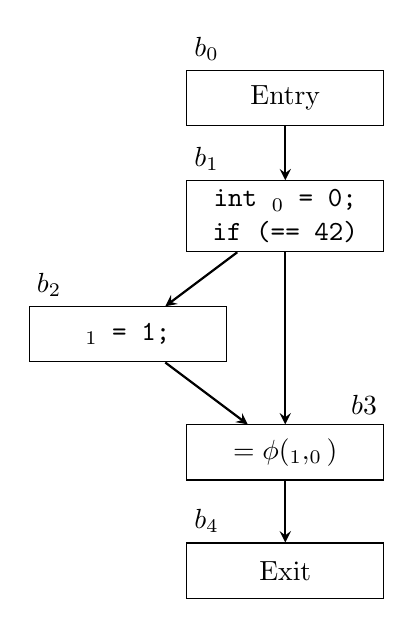
\begin{tikzpicture}
                \tikzstyle{node} = [rectangle, minimum width=2.5cm, minimum height=.7cm, text centered, draw=black, node distance=1.5cm]
                \tikzstyle{arrow} = [thick,->,>=stealth]
                
                \node (entry) [node, label={[xshift=-1cm]$b_0$}] {Entry};
                \node (b1) [node, below of=entry, align=center, label={[xshift=-1cm]$b_1$}] {\texttt{int $\mOut_0$ = 0;} \\ \texttt{if (\In == 42)}};
                \node (b2) [node, below of=b1, xshift=-2cm, label={[xshift=-1cm]$b_2$}] {\texttt{$\mOut_1$ = 1;}};
                \node (b3) [node, below of=b2, xshift=+2cm, align = center, label={[xshift=1cm]$b3$}] {$\mOut = \phi(\mOut_1, \mOut_0)$};
                \node (exit) [node, below of=b3, label={[xshift=-1cm]$b_4$}] {Exit};

                \draw [arrow] (entry) -- (b1);
                \draw [arrow] (b1) -- (b2);
                \draw [arrow] (b1) -- (b3);
                \draw [arrow] (b2) -- (b3);
                \draw [arrow] (b3) -- (exit);
            \end{tikzpicture}
        \caption{Control Flow Graph}
        \label{fig:cfg}
    \end{subfigure}\hfill
    \begin{subfigure}[t]{.45\textwidth}
        \centering
        \begin{tikzpicture}
            \tikzstyle{node} = [ellipse, minimum width=2.5cm, minimum height=.7cm, text centered, draw=black, node distance=2cm]
            \tikzstyle{arrow} = [thick,->,>=stealth]
            
            \node (b1) [node] {\texttt{int $\mOut_0$ = 0;}};
            \node (b2) [node, below left of=b1] {\texttt{\In == 42}};
            \node (b3) [node, below of=b2] {\texttt{$\mOut_1$ = 1;}};
            \node (b33) [node, below right of=b3] {$\mOut = \phi(\mOut_1, \mOut_0)$};

            \draw [arrow] (b1) -- (b33);
            \draw [arrow, blue] (b2) -- (b3);
            \draw [arrow] (b3) -- (b33);
        \end{tikzpicture}
        \caption{Program Dependence Graph\\The black edges are data dependencies, while blue edges show control dependencies}
        \label{fig:pdg}
    \end{subfigure}
    \caption{Different graph representations for the program in \ref{fig:ifEx}}
\end{figure}


\section{Program Slicing}

\com{put in new section: static techniques? could also include some stuff about what nildumu does}

Slicing is a technique used to find those sections of a program, that are influenced by (forward slice) or influence (backward slice) a given location in the program \cite{weiser81}.
This location is called the \emph{slicing criterion} and is a tuple $\langle s, v \rangle$ of a program statement $s$ and a variable $v$.
The \emph{backward slice} with respect to the criterion $\langle s, v \rangle$ contains all statements that influence the value of $v$ at point $s$ in the program. 
A \emph{forward slice} with respect to the criterion $\langle s, v \rangle$ contains all statements that are influenced by the value of $v$ assigned at point $s$ in the program.

Computing a program slice can be efficiently done using the PDG of the given program. Since all dependencies are explicitly represented as edges, the computation of a program slice is reduced to a reachability problem \cite{ottenstein84}: 

The backward slice for a node $v$ is given as the set of all nodes $v'$, for which a path $v' \stackrel{*}{\rightsquigarrow} v$ exists. The forward slice of node $v$ is given as the set of all nodes $v'$, for which a path $v \stackrel{*}{\rightsquigarrow} v'$ exists.

Horwitz \cite{horwitz88sdg} noted that interprocedural slices could be computed similarly using system dependence graphs.

Tools like JOANA use slicing techniques on system dependence graphs to analyse the information flow in programs and give non-interference guarantees where possible \cite{hammer09}.

\begin{figure}
    \centering
    \begin{minipage}{.4\textwidth}
        \begin{algorithm}[H]
            \hspace*{\algorithmicindent} \textbf{Input} \In: int \\
            \hspace*{\algorithmicindent} \textbf{Output} sum, product: int \\
            \hspace*{.5em}
            \begin{algorithmic}
                \State $i: int \leftarrow 0$
                \State $sum: int \leftarrow 0$
                \State $product: int \leftarrow 1$
                \While{$i \leq \mIn$}
                    \State $sum \leftarrow sum + i$
                    \State $product \leftarrow product * i$
                    \State $i++$
                \EndWhile\\
                \Return
            \end{algorithmic}
        \end{algorithm}
    \end{minipage}
    \hfill
    \begin{minipage}{.4\textwidth}
        \begin{algorithm}[H]
            \hspace*{\algorithmicindent} \textbf{Input} \In: int \\
            \hspace*{\algorithmicindent} \textbf{Output} sum, product: int \\
            \hspace*{.5em}
            \begin{algorithmic}
                \State $i: int \leftarrow 0$
                \State $sum: int \leftarrow 0$
                \State $\color{white} product: int \leftarrow 1$
                \While{$i \leq \In$}
                    \State $sum \leftarrow sum + i$
                    \State $\color{white} product \leftarrow product * i$
                    \State $i++$
                \EndWhile\\
                \Return
            \end{algorithmic}
        \end{algorithm}
    \end{minipage}
    \caption{The right side shows a backward slice of the function on the left for the slicing criterion $\langle \text{return}, \: sum \: \rangle$}
    \label{fig:slice}

\end{figure}


\section{Model Counting}

Given a propositional formula $F$, the model counting problem (\#SAT) is the problem of finding the number of distinct variable assignments for $F$, for which $F$ evaluates to true \cite{biere09}. So the solution for the formula shown in  \ref{fig:satEx} is \#F = 3, with the fulfilling variable assignments being $\{ x = \mttt, y = \mfff\}, \{x = \mttt, y = \mttt\}$ and  $\{x = \mfff, y = \mfff\}$. We will denote the model count of a propositional formula $f$ as $mc(f)$.

\#SAT is a generalization of the SAT problem and falls into the \#P-complete complexity class, as demonstrated by Valiant in \cite{valiant79}.

Early exact model counting techniques, such as \cite{birnbaum99}, or the well-known tool sharpSAT \cite{thurley06} use a DPLL-style exploration of the solution space. Another class of model counters instead employ complex transformations to turn the given CNF formula into a different representation, which makes model counting a far easier problem. Common are transformations into \emph{binary decision diagrams} \cite{bdd} or \emph{deterministic, decomposable negation normal form} \cite{darwiche01}. An example of such a model counter is the \texttt{c2d} tool by Darwiche \cite{darwiche04}.

\paragraph*{Approximate Model Counting}
State-of-the-art exact model counters scale to a couple of hundred variables.  This limit can be pushed to around 1,000 variables if we allow approximate solutions \cite{biere09}.
The first approximate \#SAT algorithm for DNF formulas was introduced by Luby and Karp in \cite{karp89} used Monte-Carlo techniques. This approach was extended to work on CNF formulas by Chakraborty, Meel and Vardi in \cite{chakraborty13}. Both procedures fall under category of $(\epsilon, \delta)$-counters: for $0 < \epsilon, \delta \leq 1$, the approximated solution $\#F_{approx}$ to the true solution of the problem \#F, lies in the interval $[(1 + \epsilon)^{-1} \#F, \: (1 + \epsilon) \#F]$ with a probability of $1 - \delta$ \cite{karp89,chakraborty13}.

\begin{figure}
    \centering
    $F := x \lor \lnot y$
    \caption{Propositional formula with 2 variables}
    \label{fig:satEx}
\end{figure}

\paragraph*{Projected Model Counting}
Given a set of propositional variables $\mathcal{V}$ and a propositional formula $F$ over $\mathcal{V}$, projected model counting (\#$\exists$SAT) is the problem of finding the number of assignments to a set of priority variables $\mathcal{P} \subseteq \mathcal{V}$, such that the assignment can be extended to an assignment over $\mathcal{V}$ that fulfills $F$. Considering the example from \ref{fig:satEx} and a priority set $\mathcal{P} = \{x\}$, the number of projected models is 2, with both possible assignments of $x$ being extendable to a fulfilling assignment over all variables by setting $y = \mfff$. We will denote the projected model count of a propositional formula $f$ over the set of priority variables $\mathcal{P}$ as $mc_\mathcal{P}(f)$.

The problem is introduced by Aziz et.al. in \cite{aziz15}, along with a discussion of approaches to solve \#$\exists$SAT. \td{finish}

% Model Counting
% Complexity
% Hashing-based approaches
% Application to CNF
% (\epsilon, \delta) approximation / "Probably Approximately Correct"

%%% relevant for this section
% The Complexity of Enumeration and Reliability Problems (Valiant '79) -- \cite{valiant79}
% A scalable approximate model counter (chakraborty '13) -- \cite{chakraborty13}

\chapter{Basic Analysis Design}\label{sec:design}

The analysis we will present in  this thesis combines static and dynamic approaches to the QIFC problem. It runs in several stages:

First is a static pre-processing stage. It identifies program parts that are critical to the flow of information and restricts the subsequent analysis to those parts.

Following the pre-processing, a dependency analysis examines possible program executions and evaluates the explicit and implicit information flow along these execution paths. We encode these information flows in propositional formulas and evaluate them using an approximate model counter. The generated boolean predicates can be used to estimate both the channel capacity of the input program as well as the dynamic leakage for a specific execution.

During the evaluation of the channel capacity, the generated boolean predicates might prove to be too complex to be evaluated by a model counter. In this case, our tool will split the program into segments. The segments are analyzed separately and the results are combined for an overall estimation of the program's channel capacity. The analysis of the segments will either be done using the previously generated boolean formulas or by the static QIFC tool Nildumu.

The analysis is integrated into an interpreter that will execute the program for a given input and, additionally to the channel capacity, will give an estimation for the dynamic leakage of the execution.

This chapter will focus on the basic principles of the dependency analysis: The generation of the boolean predicates and the relation between those predicates and the amount of information leaked by the program. For this, we assume that input programs have no loops and no function calls. How these structures can be handled is discussed in section \ref{ch:loops}.

\section{Input Programs}\label{sec:inputLang}

Input programs are written in a variant of the \texttt{while}-language with functions. The language contains the following control structures, using their standard semantics:

\begin{multicols}{2}
    \begin{itemize}
    \setlength\itemsep{0em}
    \item sequential composition
    \item assignments
    \item \texttt{if}-statements
    \item \texttt{while}-statements
    \item \texttt{break}-statements
    \item (recursive) function calls
\end{itemize}
\end{multicols}



The right-hand side of an assignment is an expression that uses the standard arithmetic and bitwise boolean operators. Boolean expressions used in \texttt{while}- and \texttt{if}-statements are defined in the standard way. As already mentioned, we disallow loops and function calls in our input programs for now.

We continue to use the notations introduced in section \ref{p:input} for the input program. Furthermore,  we denote the set of all statements (expressions) that are part of the language as $\stmts$ ($\expr$). Subscripts, such as $\stmts_q$ ($\expr_q)$ indicate the set of statements (expressions) that belong to the program part $q$, where $q$ could be a loop, a function, or the program as a whole.

In our analysis, we work with the input's CFG as well as the PDG, both in SSA form. To further navigate the data structures, we use the following definitions:

\begin{definition}[CFG predecessors and successors]\label{def:succPred}
    The functions will return the set of predecessor and successor blocks respectively for the given basic block.
    \begin{align*}
        pred &: \: \bb_p \to 2^{\bb_p}\\
        succ &: \: \bb_p \to 2^{\bb_p}
    \end{align*}
    We assume for $pred(b)$ that the returned set of predecessors for $b$ is ordered and that the order corresponds to the arguments of any $\phi$-functions that might be present in $b$.
\end{definition}

\begin{definition}
    Let $p$ be a program with statements $\stmts_p$ and basic blocks $\mbb_p$. The function
    \begin{center}
        $BB_p: \: \stmts_p \to \mbb_p$
    \end{center}
    returns for every statement $s \in \stmts_p$ the basic block $b \in \bb_p$ that contains the statement $s$.
\end{definition}

\begin{definition}
    Let $p$ be a program with statements $\stmts_p$ and values \val$_p$. The function
    \begin{center}
        $def: \: $\val$_p \to \stmts_p$
    \end{center}
    returns for every $v \in$ \val$_p$ the statement $s \in \stmts_p$, where the value $v$ is defined. Due to $p$ being in SSA form, this location is unique.
\end{definition}

In our analysis, we view all values as bit vectors. All values are signed integers of a fixed width $w$. We represent the numerical value of an integer as a bit vector using the following map:

\begin{definition}[Bit vector]
    The function
    \begin{center}
        $bv: \:  \mathbb{Z} \to \{0, 1\}^w$
    \end{center}
    maps integers to bit vectors of length $w$, where $bv(n)$ is the two's complement representation of the integer $n$.
    The returned value $bv(n)$ is subject to possible over- or underflows, should the number $n$ not be representable as a $w$-bit two's complement number.
\end{definition}

\paragraph{Execution Value}
We alter the definition of $\llbracket p \rrbracket_h: \{L\} \to \mathcal{L}$ to a function 
\begin{center}
    $\llbracket p \rrbracket_h: \: \val_p \to \{0, 1\}^w \cup \{\bot\}$
\end{center} that takes a program value as an argument and returns the numerical value that was assigned during the execution with input $h$. The numerical value is given as a bit vector of the number's two's complement. If in this execution, the value remains undefined, because the corresponding assignment instruction wasn't executed, the function will return $\bot$. Because the program $p$ does not contain loops or function calls, no assignment can be executed more than once. Thus, $\llbracket p \rrbracket_\cdot(\cdot)$ is well-defined.



\section{Foundations of Dependency Analysis}\label{sec:prop}

The aim of the dependency analysis is to generate a vector of propositional formulas for each program value that we call the \emph{dependency vector}.  This vector contains a formula for each bit of the value, that encodes the state of the bit depending on the bits of the input value. More specifically, the formula contains variables that represent the bits of the input value and if we initialize these variables with the bits of an input, the dependency vector of a value will evaluate to its execution value.

\paragraph{Introductory Example}\label{p:intro}
Before giving a detailed explanation of our analysis, we will demonstrate the basic principles in a short example. The program we want to analyze is shown in figure \ref{fig:introEx}. The program takes an input value, performs two bitwise operations on the value, and then leaks the result. 

\begin{figure}
    \centering
    \begin{minipage}{.7\linewidth}
        \begin{algorithm}[H]
            \hspace*{\algorithmicindent} \textbf{Input} \In $:= (\mIn^2 \mIn^1 \mIn^0)$: int \\
            \hspace*{\algorithmicindent} \textbf{Output} $\mOut_1$: int
            \hspace*{1em}
            \begin{algorithmic}[1]
                \State $\mOut_0 \leftarrow \mIn \; \& \; 110_2 \: \: \: \textcolor{blue}{[H^2 \: H^1 \:0]}$
                \State $\mOut_1 \leftarrow \mOut_0 \; | \; 010_2 \: \: \: \textcolor{blue}{[H^2 \: 1 \: 0]}$
            \end{algorithmic} 
        \end{algorithm}
\end{minipage}
\caption{Introductory example program. Behind each line of code, we have written the propositional vector that represents the assigned value}
\label{fig:introEx}
\end{figure}

Analyzing the program line by line, we can formulate conditions for the assigned values that depend on the values and operations used in the assignment expression:
\begin{itemize}
    \item On line 1, the program assigns to the value $L_0$ the result of a bitwise \texttt{\&}-operation. The right-hand operand is a constant. Because the least significant bit of this constant is \texttt{0}, the least significant bit of $L_0$ must also be \texttt{0}. The two left-hand bits of $L_0$ are identical to the corresponding bits in \In. Thus, we can describe the value $L_0$ by the vector $[H^2 \: H^2 \: 0]$.
    \item On line 2, using the same approach as above, we can ascribe to the value $L_1$ the vector $[H^2 \: 1 \: 0]$
\end{itemize}

The dependency vector $[H^2 \: 1 \: 0]$ which we computed for the output value $\mOut_1$, describes all possible output values of the example program. The vector shows that the last two bit of the output are constant and that the most significant bit is equal to the most significant bit of the input. From this information, we can conclude the following:
\begin{itemize}
    \item The \emph{channel capacity} of the example program is $\log_2(2) = 1$, because the program has only two possible outputs: $\mathtt{110}_2$ iff the most significant bit of \In is \texttt{1} and $\mathtt{010}_2$ iff the most significant bit of \In is \texttt{0}.
    \item Given the value of $\mOut_1$ after an execution, we can infer the value of the most significant bit of $\mIn$. We have no information about the other two bits. For any possible output $l = (l^2 l^1 l^0)$, its indistinguishability set is given by $\mathcal{H}_l := \{ (h^2 h^1 h^0) \in \{0, 1\}^3 \: | \: l^2 = h^2\}$. The \emph{dynamic leakage} of a single execution is $\log_2(2^3) - \log_2(2^2) = 1$.
\end{itemize}

\paragraph{Basic Definitions and Notation}
Propositional formulas are made up of boolean constants \bool \: = $\{ \mttt, \mfff \}$, boolean variables $b_i \in $ \textsc{Var}$_\mbool$ and the standard boolean operators $\{ \lnot, \land, \lor, \implies, \iff \}$. \: \bform{} is the set of all boolean formulas over \textsc{Var}$_\mbool$.

In order to relate bit-vectors and propositional formulas to each other, we use the following definitions:

\begin{definition}[Mapping Bits to Boolean Constants]\label{def:b}
The bijective map $\mathcal{B}: \{0, 1\} \to  \mbform$ maps a bit to a boolean constant.
    \begin{center}
    $\mathcal{B}: \{0, 1\} \to \mbform$
    \begin{align*}
        0 &\mapsto \mfff\\
        1 &\mapsto \mttt
    \end{align*}
    \end{center}
Throughout this thesis, we will apply $\mathcal{B}(\cdot)$ and $\mathcal{B}^{-1}(\cdot)$ implicitly where needed.
\end{definition}

\begin{definition}[Mapping Values to Vectors of Boolean Variables]
    The map
    \begin{center}
        $\var: \: \val_p \to  \mbform^w$
    \end{center}
     assigns a vector of fresh propositional variables to a program value. Each boolean variable is used to represent a bit of the value. A boolean variable is fresh if it is not yet used to represent any other bit. This means that for values $v_0 \neq v_1 \in \val_p$ we have $\var(v_0) \cap \var(v_1) = \emptyset$.
\end{definition}
We will later use the function $\var(\cdot)$ to instantiate propositional variable vectors that represent the input value(s) of the program we are analyzing. The dependency vectors we compute are based on the variable set of these variable vectors. They form the so-called \emph{independent set}:

\begin{definition}[Independent Set]
    Let $\{ \mIn_0, ..., \mIn_m \}$ be the set of input values of \pp. The set of boolean variables
    \begin{center}
        $\var_p := \bigcup\limits_{i \in \{1,..., m\}} \var(\mIn_i)$
    \end{center}
    is called the independent set. The independent set defines the variables that are used in propositional formulas during the analysis.
\end{definition}

\paragraph{Dependency Analysis for Explicit Information Flow}

In the introductory example we introduced the idea of the \emph{dependency vector}: A vector of propositional formulas that represents the state of the value's bits in terms of the bits of the input value. In this section, we will explain how the dependency vector can be computed.

\begin{definition}[Expression Evaluation and Dependency Vectors]\label{def:exprEval}
     The function
    \begin{center}
        $\mathcal{E}: \: \expr \to \mbform^w$
    \end{center}
    evaluates program expressions and computes a vector of propositional formulas that represent the expression result. The computation of $\mathcal{E}(e)$ is shown in figure \ref{fig:expr}.
\end{definition}

\begin{definition}[Dependency Vector]
        The \emph{dependency vector} function maps each value to a vector of propositional formulas. For a value $v$ that is defined in a statement as $v := e$, we define:
    \begin{center}
        $dVec: \: \val_p \to \mbform^w$,\\
        $dVec(v) := \mathcal{E}(e)$
    \end{center}
    The map is well-defined since $p$ is given in SSA-form which means that each value is defined exactly once. We use $dVec(v)^i$ to mean the i-th entry of the vector $dVec(v)$.
    \end{definition}

\begin{figure}
    \begin{subfigure}{1\textwidth}
    \centering
        Let $e := n, \quad n \in \mathbb{Z}$\\
        $\mathcal{E}(e) := \mathcal{B}(bv(n))$
        \caption{Constant Values are represented by dependency vectors that contain boolean constants. The vector entries correspond to the two's complement representation of the constant's numerical value.}
    \end{subfigure}
    \bigskip
    \begin{subfigure}{1\textwidth}
        \centering
        Let $e := \mIn$\\
        $\mathcal{E}(e) := \var(\mIn)$
        \caption{Input parameters are represented by a vector of boolean variables. The variables are part of the independent set $\var_p$ of $p$ and dependency vectors of non-input variables are defined as a function of these variables.}
    \end{subfigure}
    \bigskip
    \begin{subfigure}{1\textwidth}
        \centering
        Let $e := v, \quad v \in \val_p$\\
        $\mathcal{E}(e) := dVec(v)$
        \caption{Variable accesses are evaluated to the dependency vector of the accessed variable.}
    \end{subfigure}
    \bigskip
    \begin{subfigure}{1\textwidth}
    \centering
    Let $e := e_0 \oplus e_1$ or $e := \oplus e_0$
       \caption{Dependency vectors of unary or binary arithmetic expressions and unary or binary bitwise boolean expressions are computed using the combinatorial logic of the two's complement. Even though this logic normally operates on bits (either \texttt{0} or \texttt{1}), we can apply the boolean operations also to propositional formulas, without changing their semantics.}
    \end{subfigure}
    \caption{Definition of $\mathcal{E}(e)$ for different types of expressions $e$}\label{fig:expr}
\end{figure}

To assign each value its dependency vector, we compute $\mathcal{E}(e)$, for the expression $e$ that defines the value in question. For accesses to input variables and constants, the evaluation of $\me{\cdot}$ is straightforward. For other expressions, the evaluation of $\mathcal{E}(e)$ usually depends on the dependency vectors of use-values of $e$. We can guarantee that the needed dependency values have previously been computed, if we evaluate the dependency vectors of program values in the order in which the values are defined in the program.

\section{Measuring Information Leakage with Dependency Vectors}\label{sec:leak}

The entries of a value's dependency vector describe on a bit level, which execution value will be assigned to the value for a certain input value. They take into account all data dependencies in the program. Therefore, we are able to capture all explicit information flows using the dependency vectors.

To demonstrate the connection between a value's dependency vector and its execution value for a particular program run, we evaluate the propositional formulas using the following truth assignment:

\begin{definition}[Evaluation of Dependency Vectors]\label{def:val}
    Every concrete input $h \in \mathcal{H}$ for the input value \In induces a truth assignment: Given the concrete input value $h$ for the input variable $\mIn$, we assign the boolean variables in $\var(\mIn)$ the values of the bits in $h$.
    The evaluation of a propositional formula $f$ with respect to the truth assignment induced by the input $h$ will be denoted by $\mathcal{V}_h (f)$.
\end{definition}

Using the truth assignment induced by a particular input $h \in \mathcal{H}$, the dependency vectors fulfill the following theorem:

\begin{theorem}[Equivalence Theorem]\label{thm:equiv}
    Given an input value $h \in \mathcal{H}$ for the program $p$, let $v$ be an arbitrary value in the program $p$. The relation between the dependency vector and the execution value of $v$ is given by:
    \begin{center}
        $\forall 0 \leq i < w: \mathcal{V}_h(dVec(v)^i) \iff \llbracket p \rrbracket_h (v)^i$
    \end{center}
    At this stage, we have not yet introduced the analysis of programs with diverging control flow. For now, the theorem can only be applied to programs with linear control flow. A proof for the theorem is given in appendix \ref{ch:proofEquiv}.
\end{theorem}

Using theorem \ref{thm:equiv}, we can compute both leakage measures with the following lemmata:

\begin{lemma}[Dynamic Leakage]
    Let $p$ be a program with the concrete value $l$ of the output variable \Out{} being leaked to a public output channel during the execution of $p$ with input $h$.
    The size of $l$'s indistinguishability set $\mathcal{H}_l$ is given by the number of models of the formula:
    \begin{center}
        $F_{dyn} : \bigwedge\limits_{0 \leq i < w} \left( \llbracket p \rrbracket_h(\mOut)^i \iff \mathcal{V}_h(dVec(\mOut))^i \right)$
    \end{center}
\end{lemma}

The formula $F_{dyn}$ contains only the boolean variables from the set $\var_p$. Each model of $F_{dyn}$ thus is a truth assignment $\beta: \var_p \to \mbool$.
If for a truth assignment $\beta$ the formula $F_{dyn}$ is fulfilled, the dependency vector of the output, evaluated with respect to this truth assignment, is equivalent to the bit vector $l$. From theorem\ref{thm:equiv}, it follows that the execution of $p$ with the input $h$ induced by $\beta$ will result in the output $l$.

Assuming a uniform distribution of $\mathcal{H}$, the dynamic leakage of the execution of $p$ with the input $h$ is given by
    \begin{center}
        $L_{dyn}(p, h) = \log_2(|\mathcal{H}|) - \log_2(mc(F_{dyn}))$
    \end{center}

\begin{lemma}[Channel Capacity]
    Let $p$ be a program with an output value \Out. Let $o := [o_0 ... o_w]$ be a vector of boolean variables with $o \cap \var_p = \emptyset$.
    
    The number of distinct outputs of $p$ is given by the projected model count of the formula
    \begin{center}
        $F_{cc} : \bigwedge\limits_{0 \leq i < w} \left( o_i \iff dVec(\mOut)^i \right)$
    \end{center}
    with the variables in $o = [o_0, ..., o_w]$ as the set of priority variables.
    Assuming a uniform distribution of $\mathcal{H}$, the channel capacity is given by
    \begin{center}
        $cc(p) = \log_2(mc_o(F_{cc}))$
    \end{center}
\end{lemma}

\section{Dependency Analysis for Implicit Information Flow}
Implicit information flow occurs when an attacker can draw conclusions about the secret inputs by observing the values of the public outputs and then reconstructing the execution path of a program execution. In this section we will extend the dependency analysis from before to include implicit information flows caused by \texttt{if}-statements. Implicit information flows from more complex control flow structures, such as loops and function calls, are discussed in chapter \ref{ch:loops}. Throughout this section, we use the program shown in figure \ref{fig:doubleIf} as an example to demonstrate the individual steps of the analysis.

\begin{figure}
\centering
\begin{minipage}{.4\linewidth}
    \begin{algorithm}[H]
        \hspace*{\algorithmicindent} \textbf{Input} \In: int \\
        \hspace*{\algorithmicindent} \textbf{Output} \Out: int
        \begin{algorithmic}[1]
            \If{$\mIn < 0$}
                \State $\mOut \leftarrow 0$
            \Else
                \State $\mIn \leftarrow \mIn - 1$
                \If{$\mIn < 0$}
                    \State $\mOut \leftarrow 1$
                \Else
                    \State $\mOut \leftarrow 2$
                \EndIf
            \EndIf
    \end{algorithmic} 
    \end{algorithm}
    \end{minipage}
    \hfill
    \begin{minipage}{.55\textwidth}
        \centering
            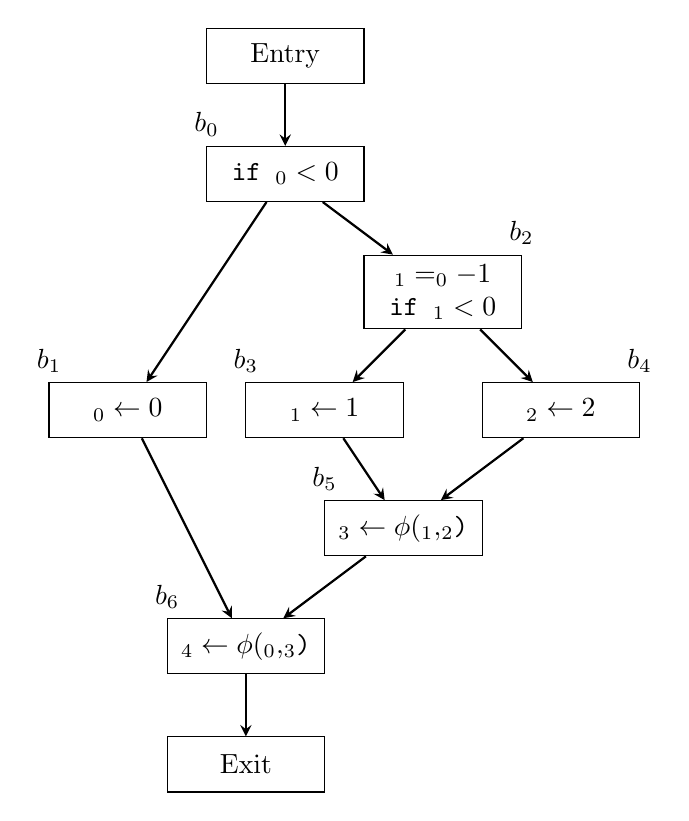
\begin{tikzpicture}
                \tikzstyle{node} = [rectangle, minimum width=2cm, minimum height=.7cm, text centered, draw=black, node distance=1.5cm]
                \tikzstyle{arrow} = [thick,->,>=stealth]
                
                \node (entry) [node] {Entry};
                \node (b1) [node, below of=entry, align=center, label={[xshift=-1cm]$b_0$}] {\texttt{if $\mIn_0 < 0$}};
                \node (b2) [node, below of=b1, xshift=-2cm, yshift=-1.5cm, label={[xshift=-1cm]$b_1$}] {\texttt{$\mOut_0 \leftarrow 0$}};
                
                \node (b3) [node, below of=b1, xshift=+2cm, align = center, label={[xshift=+1cm]$b_2$}] {$\mIn_1 = \mIn_0 - 1$\\\texttt{if $\mIn_1 < 0$}};
                
                \node (b4) [node, below of=b3, xshift=-1.5cm, label={[xshift=-1cm]$b_3$}] {\texttt{$\mOut_1 \leftarrow 1$}};
                \node (b5) [node, below of=b3, xshift=+1.5cm, label={[xshift=+1cm]$b_4$}] {\texttt{$\mOut_2 \leftarrow 2$}};
                \node (b6) [node, below of=b5, xshift=-2cm, label={[xshift=-1cm]$b_5$}] {\texttt{$\mOut_3 \leftarrow
                \phi(\mOut_1, \mOut_2$)}};
                
                \node (b7) [node, below of=b6, xshift=-2cm, label={[xshift=-1cm]$b_6$}] {\texttt{$\mOut_4 \leftarrow
                \phi(\mOut_0, \mOut_3$)}};
                \node (exit) [node, below of=b7] {Exit};

                \draw [arrow] (entry) -- (b1);
                \draw [arrow] (b1) -- (b2);
                \draw [arrow] (b1) -- (b3);
                \draw [arrow] (b2) -- (b7);
                \draw [arrow] (b3) -- (b4);
                \draw [arrow] (b3) -- (b5);
                \draw [arrow] (b4) -- (b6);
                \draw [arrow] (b5) -- (b6);
                \draw [arrow] (b6) -- (b7);
                \draw [arrow] (b7) -- (exit);
            \end{tikzpicture}
    \end{minipage}\hfill
    \caption{Program text and CFG of a short example program. The program returns 0 if $\mIn < 0$, 1 if $\mIn == 0$ and 2 otherwise. The CFG is in SSA-form.}
    \label{fig:doubleIf}
\end{figure}

To include implicit information flow in the analysis, we develop the function $exec: \: \mbb_p \to \mbform$ that assigns each basic block $b$ of a program a propositional formula $exec(b)$ that is fulfilled by the inputs iff the block $b$ is executed. 

In a CFG, the edges represent the jumps between basic blocks. We define the edge condition function $follow: \: \mbb_p \times \mbb_p \to \mbform$ to annotate CFG edges with expressions, that describe when the jump between the two blocks is taken during an execution. The edge annotations are given as propositional formulas, that already take into account the dependency vectors that were computed for the operands. Figure \ref{ex:ec} shows the CFG of the example program \ref{fig:doubleIf} with edges being annotated with their edge conditions.


% might need this later somewhere, not sure
%\begin{definition}[Jump Expression]
 %   For each basic block $b \in \mbb_p$, we define $jump(b)$ as the program expression that decides which successor block of $b$ will be executed.
 %   \begin{center}
 %       $jump: \: \mbb_p \to \mathtt{Expr}$
 %   \end{center}
 %   If $b$ ends in a conditional jump, $jump(b)$ is the expression of the conditional jump instruction.
    
 %   If $b$ ends in an unconditional jump or $b$ is the \texttt{exit} block, we define $b$ as the constant expression \ttt.
%\end{definition}

%\begin{definition}[Edge Condition]
%    Let $CFG(p) = (\mbb_p, E)$ be the CFG of the program $p$.We define
%    \begin{center}
%        $follow: E \to \mbform$\\
%        $(b_0, b_1) \mapsto 
%        \begin{cases}
%            \mathcal{E}(jump(b_0)) & \text{if the execution follows $e$ for $jump(b_0) = \mttt$}\\
%            \lnot \mathcal{E}(jump(b_0)) & \text{if the execution follows $e$ for $jump(b_0) = \mfff$}
%        \end{cases}$
%    \end{center}
%    For every edge $e := (b_0, b_1) \in E$, the propositional formula $follow(e)$ is true iff the control flow during an execution of $p$ jumps from $b_0$ to $b_1$.
%\end{definition}

\begin{figure}
    \centering
                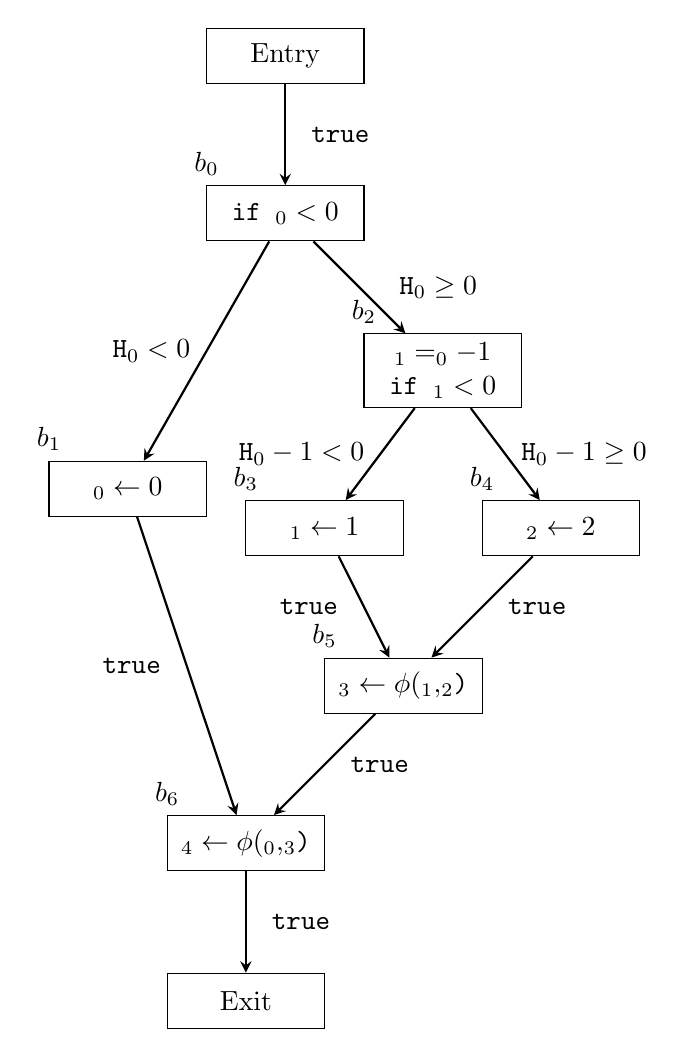
\begin{tikzpicture}
                \tikzstyle{node} = [rectangle, minimum width=2cm, minimum height=.7cm, text centered, draw=black, node distance=2cm]
                \tikzstyle{arrow} = [thick,->,>=stealth]
                
                \node (entry) [node] {Entry};
                \node (b1) [node, below of=entry, align=center, label={[xshift=-1cm]$b_0$}] {\texttt{if $\mIn_0 < 0$}};
                \node (b2) [node, below of=b1, xshift=-2cm, yshift=-1.5cm, label={[xshift=-1cm]$b_1$}] {\texttt{$\mOut_0 \leftarrow 0$}};
                
                \node (b3) [node, below of=b1, xshift=+2cm, align = center, label={[xshift=-1cm]$b_2$}] {$\mIn_1 = \mIn_0 - 1$\\\texttt{if $\mIn_1 < 0$}};
                
                \node (b4) [node, below of=b3, xshift=-1.5cm, label={[xshift=-1cm]$b_3$}] {\texttt{$\mOut_1 \leftarrow 1$}};
                \node (b5) [node, below of=b3, xshift=+1.5cm, label={[xshift=-1cm]$b_4$}] {\texttt{$\mOut_2 \leftarrow 2$}};
                \node (b6) [node, below of=b5, xshift=-2cm, label={[xshift=-1cm]$b_5$}] {\texttt{$\mOut_3 \leftarrow
                \phi(\mOut_1, \mOut_2$)}};
                
                \node (b7) [node, below of=b6, xshift=-2cm, label={[xshift=-1cm]$b_6$}] {\texttt{$\mOut_4 \leftarrow
                \phi(\mOut_0, \mOut_3$)}};
                \node (exit) [node, below of=b7] {Exit};

                \draw [arrow] (entry) -- (b1) node[midway, xshift=.7cm] {\texttt{true}};
                \draw [arrow] (b1) -- (b2) node[midway, xshift=-.7cm] {$\mathtt{H}_0 < 0$};
                \draw [arrow] (b1) -- (b3) node[midway, xshift=1cm] {$\mathtt{H}_0 \geq 0$};
                \draw [arrow] (b2) -- (b7) node[midway, xshift=-.7cm] {\texttt{true}};
                \draw [arrow] (b3) -- (b4) node[midway, xshift=-1cm] {$\mathtt{H}_0 - 1 < 0$};
                \draw [arrow] (b3) -- (b5) node[midway, xshift=1cm] {$\mathtt{H}_0 - 1 \geq 0$};
                \draw [arrow] (b4) -- (b6) node[midway, xshift=-.7cm] {\texttt{true}};
                \draw [arrow] (b5) -- (b6) node[midway, xshift=.7cm] {\texttt{true}};
                \draw [arrow] (b6) -- (b7) node[midway, xshift=.7cm] {\texttt{true}};
                \draw [arrow] (b7) -- (exit) node[midway, xshift=.7cm] {\texttt{true}};
            \end{tikzpicture}
    \caption{CFG from figure \ref{ex:ec} with annotated edges. The annotations represent the formulas $follow(e)$. For easier reading the formulas are given as propositional formulas with linear integer arithmetic instead of bit vector logic.}
    \label{ex:ec}
\end{figure}

\paragraph{Execution Conditions for Basic Blocks}
A basic block $b$ in a program is executed, iff one of its predecessor blocks is executed and the condition for execution to jump from said predecessor to the block $b$ is fulfilled. A special case is a program's entry block, which is executed in every run. This leads to the following definition: 

\begin{definition}[Execution Condition]\label{def:exec}
    For every basic block $b \in \: \mbb_p$, we define its execution condition as:
    \begin{center}
        $exec: \mbb_p \to \mbform$\\
        \begin{align*}
            exec &: BB_p \to \mathcal{F}\\
            exec(b) &:= \begin{cases}
                \mttt &  b = \mathtt{entry}\\
                \bigvee\limits_{p \: \in \: pred(b)} \left( follow(p, b) \land exec(p) \right) & \text{otherwise}\\
        \end{cases}\\
        \end{align*}
    \end{center}
\end{definition}

\begin{lemma}[Basic Block Execution]\label{lemma:exec}
    For every basic block $b \in \: \mbb_p$ and its execution condition $exec(b)$, \\ $\mathcal{V}_h(exec(b)) = \mttt \iff \text{basic block $b$ is executed in a program run with input h}$.
\end{lemma}
The proof for the lemma is given in appendix \ref{ch:proofEquiv} in conjunction with the proof for theorem \ref{thm:equiv}.
\paragraph{Example Computation}
Table \ref{tab:exec} shows the execution conditions of all the basic blocks of example \ref{fig:doubleIf}. We show how these results were computed in detail for blocks $b_3$ and $b_5$:
\begin{itemize}
    \item Basic block $b_3$ has one predecessor $b_2$ with $exec(b_2) = \mIn_0 \geq 0$. The edge $(b_2, b_3)$ represents a conditional jump that is taken iff the condition $follow((b_2, b_3)) := \mIn_0 - 1 < 0$ is fulfilled.
    \begin{align*}
        exec(b_3) &:= follow((b_2, b_3)) &&\land&& exec(b_2) \\
        &= \mIn_0 \geq 0 &&\land&& \mIn_0 - 1 < 0 \\
    \end{align*}
    
    \item Basic block $b_5$ has two predecessors $b_3$ and $b_4$. Their execution conditions are given in table \ref{tab:exec}. Both incoming edges of $b_5$ represent unconditional jumps, thus their edge conditions evaluate to $\mttt$.
    \begin{alignat*}{2}
        exec(b_5) \quad &:= follow((b_3, b_5)) \land exec(b_3) \quad &\lor & \quad follow((b_4, b_5)) \land exec(b_4)\\
        &= \mttt \land (\mIn_0 \geq 0 \land \mIn_0 - 1 < 0) &\lor & \quad \mttt \land (\mIn_0 \geq 0 \land \mIn_0 - 1 \geq 0)\\
        &= \mIn_0 \geq 0 \land (\mIn_0 - 1 < 0 \lor \mIn_0 - 1 \geq 0) \\
        &= \mIn_0 \geq 0
    \end{alignat*}
\end{itemize}

\begin{figure}
    \centering
    \begin{tabular}{ |c|c| } 
        \hline
        $b$ & $exec(b)$ \\
        \hline
        $\mathtt{entry}$ & $\mttt$ \\
        $b_0$ & $\mttt$ \\
        $b_1$ & $\mathtt{H}_0 < 0$ \\
        $b_2$ & $\mathtt{H}_0 \geq 0$ \\
        $b_3$ & $\mathtt{H}_0 \geq 0 \land \mathtt{H}_0 - 1 < 0$ \\
        $b_4$ & $\mathtt{H}_0 \geq 0 \land \mathtt{H}_0 - 1 \geq 0$ \\
        $b_5$ & $\mathtt{H}_0 \geq 0$ \\
        $b_6$ & $\mttt$ \\
        $\mathtt{exit}$ & $\mttt$ \\
        \hline
    \end{tabular}
    \caption{Evaluation of $exec(\cdot)$ for the basic blocks of program \ref{fig:doubleIf}}
    \label{tab:exec}
\end{figure}

\paragraph{Combining Implicit and Explicit Information Flows in $\phi$-functions}
The execution conditions introduced in the previous section can be used to evaluate which basic blocks will be executed depending on the inputs. They contain all control flow dependencies that are present in the program. The formulas describing the implicit flows are integrated into the dependency vectors when a value is assigned the result of a $\phi$-function. Let the value $v_2$ be defined via $v_2 := \phi(v_0, v_1), \: v_0, v_1 \in \val_p$. The assignment expression is part of basic block $b_2$ with predecessors $\{b_0, b_1\}$. The situation is shown in figure \ref{fig:phi}.

To evaluate the $\phi$-expression and compute the dependency vector for value $v_2$, we use the ternary operator $\mathbb{IF}(\cdot, \cdot, \cdot)$:

\begin{definition}[Ternary Operator]
    We define the ternary operator $\mathbb{IF}(\cdot, \cdot, \cdot)$ as:
    \begin{center}
        $\mathbb{IF}: \mbform \times \mbform \times \mbform \to \mbform$\\
        $\mathbb{IF}(c, x, y) := (c \implies x) \land (\lnot c \implies y)$
    \end{center}
    We canonically extend the definition to include propositional vectors:
    \begin{center}
        $\mathbb{IF}: \mbform \times \mbform^k \times \mbform^k \to \mbform^k$\\
        $\mathbb{IF}(c, x, y) := [\mathbb{IF}(c, x^i, y^i)]_{i = 0}^k$
    \end{center}
\end{definition}

The dependency vector of the value $v_2$ can then be computed using the definition of $\mathcal{E}(\cdot)$ for $\phi$-functions given in figure \ref{fig:exprPhi}. The correctness of this definition follows from the following considerations:

If we compute the dependency vector $dVec(v_2) := \mathcal{E}(\phi(v_0, v_1))$ of the value $v_2$, we can assume that the basic block $b_2$ is executed. Otherwise, any assignment to $v_2$ and the information contained in the assignment is irrelevant for the leakage analysis of the execution in question.

If the basic block $b_2$ is executed, at least one of its predecessors $b_0, \: b_1$ must have been executed as well for the execution to reach $b_2$. Furthermore it is impossible for both of $b_2$'s predecessors to have been executed, since so far we only consider loop-free programs, which have no back-edges in their CFG. It follows that the condition $exec(b_0) \veebar exec(b_1)$ must hold for any input value. It is therefore sufficient to check the execution condition of $b_0$ in the definition of $\mathcal{E}(\phi(v_0, v_1))$.

\begin{figure}
\begin{subfigure}{.4\textwidth}
    \centering
    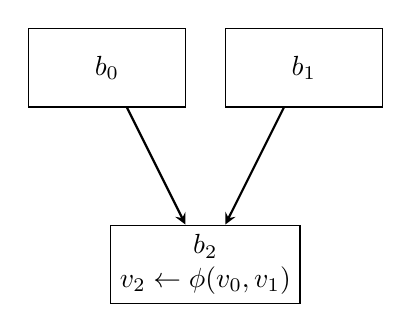
\begin{tikzpicture}
        \tikzstyle{node} = [rectangle, minimum width=2cm, minimum height=1cm, text centered, draw=black, node distance=2.5cm]
        \tikzstyle{arrow} = [thick,->,>=stealth]
                
                \node (b1) [node] {$b_0$};
                \node (b2) [node, right of=b1] {$b_1$};
                \node (b0) [node, below of=b1, xshift=1.25cm, align=center] {$b_2$ \\ $v_2 \leftarrow \phi(v_0, v_1)$};
                
                \draw[arrow] (b1) -- (b0);
                \draw[arrow] (b2) -- (b0);
                
    \end{tikzpicture}
    \caption{Section of a CFG that contains a $\phi$-function.}
    \label{fig:phi}
\end{subfigure}
\hfill
\begin{subfigure}{.5\textwidth}
\vspace{1cm}
    \begin{equation*}
\mathcal{E}(\phi(v_0, v_1)) := \mathbb{IF}(exec(b_0), v_0, v_1)
\end{equation*}
\vspace{1cm}
\caption{Extension of the definition of $\mathcal{E}(\cdot)$ in \ref{fig:expr} for the evaluation of $\phi$-functions.}\label{fig:exprPhi}
\end{subfigure}
\caption{Handling of $\phi$-functions during the dependency analysis}
\end{figure}

\paragraph{Example (cont'd)}
We complete the dependency analysis of the example program \ref{fig:doubleIf} using the algorithm shown in figure \ref{alg:depAna}. The algorithm returns the dependency vector of the leaked value. Figure \ref{fig:exFinished} shows the dependency vectors of all program values. In SSA-form, $\mOut_4$ is the value that corresponds to the program's output. The algorithm returns:
\begin{align*}
    dVec(\mOut_4) &= \mathbb{IF}(\mIn_0 < 0, dVec(\mOut_0), dVec(\mOut_3)) \\
    &= \mathbb{IF}(\mIn_0 < 0, 0, \mathbb{IF}(\mIn_0 \geq 0 \land (\mIn_0 - 1) < 0, dVec(\mOut_1), dVec(\mOut_2))) \\
    &= \mathbb{IF}(\mIn_0 < 0, 0, \mathbb{IF}(\mIn_0 \geq 0 \land (\mIn_0 - 1) < 0, 1, 2))
\end{align*}

\begin{figure}
    \centering
    \begin{algorithm}[H]
        \hspace*{\algorithmicindent} \textbf{Input} $CFG(p) = (\mbb_p, \: E):$ CFG of input program $p$ in SSA form.\\ 
        \hspace*{\algorithmicindent} \textbf{Output} $leaked: \mbform^w$\\
        \begin{algorithmic}[1]
            \State $blocks: (\mbb_p \to \mbform)$
            \State $dVec: (\val_p \to \mbform^w)$
            
            \For{$b \in \mbb_p$ in topological order}
                \State $blocks(b) \leftarrow exec(b)$
                \For{$v := e \in Statements(b)$}
                    \State $dVec(v) \leftarrow \mathcal{E}(e)$
                \EndFor
            \EndFor
            \State $leaked \leftarrow dVec(\mOut)$
    \end{algorithmic} 
    \caption{Dependency Analysis}
\end{algorithm}
    \caption{Algorithm for the dependency analysis of call-free, loop-free programs}
    \label{alg:depAna}
\end{figure}


\begin{figure}
    \centering
    \begin{tikzpicture}
                \tikzstyle{node} = [rectangle, minimum width=2cm, minimum height=.7cm, text centered, draw=black, node distance=3cm]
                \tikzstyle{arrow} = [thick,->,>=stealth]
                
                \node (entry) [node] {Entry};
                \node (b1) [node, below of=entry, align=center, label={[xshift=-1cm]$b_0$}] {\texttt{if $\mIn_0 < 0$}};
                \node (b2) [node, below of=b1, xshift=-2cm, yshift=-1.5cm, label={[xshift=-1cm]$b_1$}] {\texttt{$\mOut_0 \leftarrow 0 \quad \color{blue}{dVec(\mOut_0) = 0}$}};
                
                \node (b3) [node, below of=b1, xshift=+5cm, align = center, label={[xshift=+1cm]$b_2$}] {$\mIn_1 = \mIn_0 - 1 \quad \color{blue}{dVec(\mIn_1) = H_0 - 1}$\\\texttt{if $\mIn_1 < 0$}};
                
                \node (b4) [node, below of=b3, xshift=-2.5cm, label={[xshift=-1cm]$b_3$}] {\texttt{$\mOut_1 \leftarrow 1 \quad \color{blue}{dVec(\mOut_1) = 1}$}};
                \node (b5) [node, below of=b3, xshift=+2.5cm, label={[xshift=+1cm]$b_4$}] {\texttt{$\mOut_2 \leftarrow 2 \quad \color{blue}{dVec(\mOut_2) = 2}$}};
                \node (b6) [node, below of=b5, xshift=-2.5cm, label={[xshift=-1cm]$b_5$}, align=center] {$\mOut_3 \leftarrow
                \phi(\mOut_1, \mOut_2)$\\$ \color{blue}{dVec(\mOut_3) = \mathbb{IF}(\mIn_0 \geq 0 \land (\mIn_0 - 1) < 0, dVec(\mOut_1), dVec(\mOut_2)) }$};
                
                \node (b7) [node, below of=b6, xshift=-5cm, label={[xshift=-1cm]$b_6$}, align=center] {$\mOut_4 \leftarrow
                \phi(\mOut_0, \mOut_3 )$\\$\color{blue}{dVec(\mOut_4) = \mathbb{IF}(\mIn_0 < 0, dVec(\mOut_0), dVec(\mOut_3)) }$};
                \node (exit) [node, below of=b7] {Exit};

                \draw [arrow] (entry) -- (b1);
                \draw [arrow] (b1) -- (b2);
                \draw [arrow] (b1) -- (b3);
                \draw [arrow] (b2) -- (b7);
                \draw [arrow] (b3) -- (b4);
                \draw [arrow] (b3) -- (b5);
                \draw [arrow] (b4) -- (b6);
                \draw [arrow] (b5) -- (b6);
                \draw [arrow] (b6) -- (b7);
                \draw [arrow] (b7) -- (exit);
            \end{tikzpicture}
    \caption{CFG of program \ref{fig:doubleIf} annotated with the dependency vectors of each program value}
    \label{fig:exFinished}
\end{figure}

\chapter{Extended Dependency Analysis}\label{ch:loops}

Chapter \ref{sec:design} introduced the basic principles of the dependency analysis and how the results of the dependency analysis can be used to measure the amount of leaked information for a given program.

In this chapter we will extend the dependency analysis to include the handling of arrays as well as more complex control flow structures, namely loops and (recursive) function calls.

\paragraph{Sequential Execution Value}
So far, we used the execution value $\llbracket p \rrbracket_h (v)$ to get the actual value of $v$ during the execution with input $h$. Allowing loops and function calls to our input programs means, that a value $v$ can now have more than one execution value during an execution, because it is possible for the statement where $v$ is defined to be executed multiple times.
To ensure that the execution value of a value is still well defined, we add a parameter $i$ that signifies, which of the possible execution values we want to refer to.

\begin{definition}[Sequential Execution Value]
    For a program $p$ and an input value $h$, we define the sequential execution value function as
    \begin{center}
        $\llbracket p \rrbracket_h: \val_p \times \mathbb{N} \to \{0, 1\} ^w \cup \{\bot\}$.
    \end{center}
    For a value $v$, $\llbracket p \rrbracket_h(v, i)$ is the numerical value of the $i$-th assignment of $v$ during the execution. If there is not $i$-th assignment of the value, the function returns $\bot$.
\end{definition}
The definition of $\llbracket p \rrbracket_h(\cdot)$ used in the previous chapter corresponds to the value $\llbracket p \rrbracket_h (\cdot, 1)$ of the new definition. We continue to use $\llbracket p \rrbracket_h(\cdot)$ for $\llbracket p \rrbracket_h (\cdot, 1)$. 

\section{Loops}
Loops are handled during the dependency analysis in the following steps:

First, we isolate the loop from the rest of the program and analyse the loop body as a separate function with distinct inputs and outputs. Second, we generate the dependency vectors for loop output values for each iteration by recursively applying the mapping from loop iteration inputs to iteration outputs to itself. Finally, we combine the iteration results into dependency vectors that represent the loop computations as a whole.

Because all three steps refer to the same program values at times, we use the following notations to differentiate them:

For a program value $v$ that is defined inside a loop $l$:
\begin{itemize}
    \setlength\itemsep{0em}
    \item $v[l]$ represents the value $v$ in the general loop body analysis.
    \item $v[l(i)]$ represents the value $v$ in the i-th iteration of the loop $l$.
    \item $v$ is the value $v$ in its state after the execution of the loop is finished
\end{itemize}

\begin{figure}
\begin{subfigure}{.5\textwidth}
    \centering
    \begin{algorithm}[H]
        \hspace*{\algorithmicindent} \textbf{Input} $\emptyset$ \\
        \hspace*{\algorithmicindent} \textbf{Output} $\mOut$: int
        \begin{algorithmic}[1]
        \State $\mOut: int \leftarrow 0$
        \State $i: int \leftarrow 1$
            \While{$\mOut \neq -1$}
                \State $\mOut \leftarrow \mOut \: | \: i$
                \State $i \leftarrow i << 1$
            \EndWhile
    \end{algorithmic} 
    \end{algorithm}
    \caption{Program code before SSA-transformation}
    \label{fig:loop}
\end{subfigure}
\hfill
\begin{subfigure}{.4\textwidth}
    \centering
    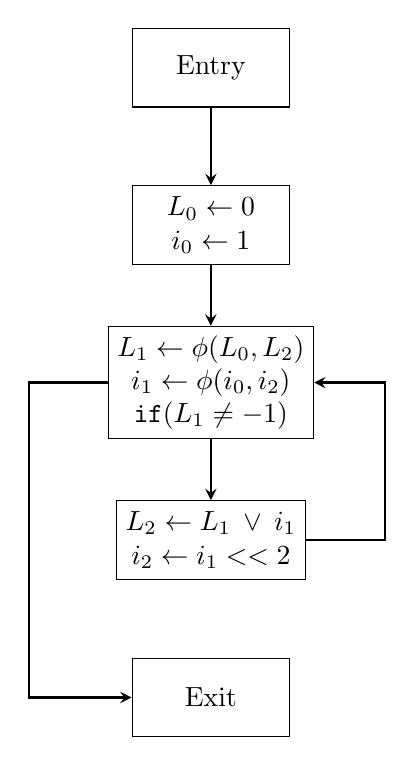
\begin{tikzpicture}
        \tikzstyle{node} = [rectangle, minimum width=2cm, minimum height=1cm, text centered, draw=black, node distance=2cm]
        \tikzstyle{arrow} = [thick,->,>=stealth]
                
                \node (entry) [node, xshift=1cm] {Entry};
                \node (b1) [node, below of=entry, align=center] {$L_0 \leftarrow 0$\\$i_0 \leftarrow 1$};
                \node (b2) [node, below of=b1, align=center] {$L_1 \leftarrow \phi(L_0, L_2)$ \\ $i_1 \leftarrow \phi(i_0, i_2)$\\ $\mathtt{if} (L_1 \neq -1)$};
                \node (b3) [node, below of=b2, align=center] {$L_2 \leftarrow L_1 \: \lor \: i_1$ \\ $i_2 \leftarrow i_1 << 2$};
                \node (exit) [node, below of=b3] {Exit};
                
                \draw[arrow] (entry) -- (b1);
                \draw[arrow] (b1) -- (b2);
                \draw[arrow] (b2) -- (b3);
                \draw[arrow] (b3.east) -- ++(1,0) |- (b2.east);
                \draw[arrow] (b2.west) -- ++(-1,0) |-(exit.west);
    \end{tikzpicture}
    \caption{CFG of the example program}\label{fig:loopEx}
    \label{fig:whilegraph}
\end{subfigure}
\caption{Example program for Loop Analysis. The program doesn't have a secret input and always returns $-1$.}
\end{figure}

\paragraph{General Loop Body Analysis}
We begin the analysis by defining input and output values for a single loop iteration. 

The set of values that are used inside a loop can be divided into two categories:
\begin{enumerate}
    \item Values, that might change with each iteration. These are values that are defined inside the loop (or before the loop in the case of the first loop iteration) and then get passed to the next iteration via a $\phi$-function in the loop head.
    \item Values, that are constant for every loop iteration.
\end{enumerate}

The first group of values represent the inputs of a loop iteration, while the second group can be treated as constants in the loop analysis, even if their concrete value is unknown. The outputs of a loop iteration are the values that are defined inside the loop and used either in the subsequent iteration or after the loop.

\begin{definition}[Loop Inputs and Outputs]
    Let $l$ be a loop in program $p$.
    \begin{itemize}
        \item[(a)] We define the set $in[l]$ of inputs of the loop as the set of values defined by $\phi$-functions in $l$.
        \item[(b)] We define the set $out[l]$ of outputs of the loop as the set of values that are defined inside the loop \emph{and} appear as arguments in a $\phi$-function in $l$.
    \end{itemize}
\end{definition}

Analogous to the notation for values, $in[l]$ and $out[l]$ refer to the input and output sets during the general loop body analysis. The in- and outputs for a specific iteration $i$ are then called $in[l(i)]$ and $out[l(i)]$.

Using the defined inputs and outputs, we can apply the principles of the dependency analysis for linear programs to the loop $l$:

We set $dVec(v[l]) = \var(v[l])$ for $v[l] \in in[l]$, i.e. we represent the values of the inputs as vectors of fresh boolean variables.

Next, we compute the dependency vectors of all values defined inside the loop. To do that we analyse the blocks $l$ in topological order.

The dependency vectors of the loop outputs $out[l]$ are made up of formulas that depend on
\begin{enumerate}
    \setlength\itemsep{0em}
    \item Variables that represent loop input bits
    \item Variables that represent program input bits
\end{enumerate}

Additional to the inputs and outputs, we define a propositional formula $exit[l]$ for the $l$, that represents the condition that must be fulfilled to jump out of the loop. The  condition $exit[l]$ is given by the condition $follow(e)$ that belongs to the edge $e$ that connects the loop header of $l$ to its outside-loop successor. Like the formulas for values in $out[l]$, $exit_l$ depends on variables from the loop inputs as well as the program inputs. 

\paragraph{Example}
Figure \ref{fig:loopEx} shows an example of a program containing a loop $l$.

The inputs of the loop are the values $L_1[l]$ and $i_1[l]$. The outputs of the loop are the values $L_2[l]$ and $i_2[l]$.

The dependency vectors of those values are:
\begin{align*}
    dVec(L_1[l]) &= [L_1^2, L_1^1, L_1^0] \\
    dVec(i_1[l]) &= [i_1^2, i_1^1, i_1^0] \\
    dVec(L_2[l]) &= [L_1^2 \lor i_1^2, L_1^1 \lor i_1^1, L_1^0 \lor i_1^0] \\
    dVec(i_2[l]) &= [i_1^1, i_1^0, 0] \\
\end{align*}

The loop condition is $enter_l = (L_1[l] \neq -1)$.

\paragraph{Computing Iterations}
In the previous paragraph, we computed dependency vectors that represent the output values of the loop using abstract values as the inputs.

In this paragraph, we use this general result, to obtain dependency vectors that represent the loop outputs after a specific iteration. The formulas in these vectors will then only depend on the program input variables and not the loop variables.

Input and output values of specific loop iterations are collected in the sets $in[l(i)]$ and $out[l(i)]$, where $i$ is the iteration count. The special case $i = 0$ refers to the program state before the loop is entered. Here we define $in[l(0)]$ as $\emptyset$ and $out[l(0)]$ as the values that computed before the loop and then used inside the loop during the first iteration. For $i > 0$ we have $out[l(i)] = in[l(i + 1)]$.

Given the dependency vectors for values in $in[l(i)]$ for some value of $i$, we can compute the dependency vectors for values in $out[l(i)]$, by substituting the variables representing values in $in[l]$ by the corresponding formula of the value in $in[l(i)]$.

\begin{definition}[Iteration Substitution]
    Let $p$ be a program with a loop starting at block $l$. We are given dependency vectors for values in $in[l(i)]$. To compute the dependency vectors for values in $out[l(i)]$, we use the substitution
    \begin{center}
        $\sigma_{l(i)} := \{h_i^j \mapsto dVec(h_i)^j | \quad h_i \in in[l(i)]\}$
    \end{center}
    and apply it to the dependency vectors of $out[l]$.
\end{definition}

The substitution $\sigma_{l(i)}$ can be applied to $exit[l]$ to obtain a formula $exit[l(i)]$ that represents the condition of whether the i-th loop iteration will be entered or not.

\paragraph{Example (cont'd)} The dependency vectors of the input and output values, as well as the loop condition, for the first iterations for the example program are presented in table \ref{tab:loop}.

\begin{table}
    \centering
    \begin{tabular}{|c|c|c|c|c|c|}
    Iteration & \multicolumn{2}{|c|}{Inputs} & \multicolumn{2}{|c|}{Outputs} & Exit Condition \\
     & $L_1[l(i)]$ & $i_1[l(i)]$ & $L_2[l(i)]$ & $i_2[l(i)]$ & $exit[l(i)]$ \\
     \hline
     $i = 0$ & - & - & $[0 0 0]$ & $[0 0 1]$ & $[000] == [111]$ \\
     $i = 1$ & $[0 0 0]$ & $[0 0 1]$ & $[0 0 1]$ & $[0 1 0]$ & $[001] == [111]$ \\
     $i = 2$ & $[0 0 1]$ & $[0 1 0]$ & $[0 1 1]$ & $[1 0 0]$ & $[011] == [111]$ \\
     $i = 3$ & $[0 1 1]$ & $[1 0 0]$ & $[1 1 1]$ & $[0 0 0]$ & $[111] == [111]$ \\
    \end{tabular}
    \caption{Dependency Vectors for the values of the sets $in[l(i)]$ and $out[l(i)]$ for the example program \ref{fig:whilegraph}.}
    \label{tab:loop}
\end{table}

\paragraph{Combining Iterations for Overall Loop Result}
To finish the loop analysis, we compute dependency vectors for the output values, that represent the loop execution as a whole.

The result values of the loop depend on the number of iterations that are executed. The case that the loop is executed exactly $i$ times is represented by the condition $upto[l(i)]$:

\begin{definition}[Loop Iterations]
    Let $p$ be a program with a loop beginning with basic block $l$.
    The propositional formula
    \begin{center}
        $upto[l(i)]: (\bigwedge\limits_{0 \leq j < i} \lnot exit[l(j)]) \land exit[l(i)]$
    \end{center}
    is a propositional formula over $\var_p$ and evaluates to true, iff for a program input $h$ the loop is executed exactly $i$ times.
\end{definition}

The formula $upto[l(i)]$ encodes the following intuition: For every $j < i$, $exit[l(j)]$ must be false, otherwise the loop execution would have been aborted before the $i$-th iteration. The condition $exit[l(i)])$ must be true, otherwise the loop would have been executed more than $i$ times.

For the final set of loop output values, we make the following observations:

If the loop is executed exactly $i$ times, the results are equal to the outputs $out[l(i)]$. Whether the loop is executed exactly $i$ times or not, can be checked via the condition $upto[l(i)]$. Continuing this observation for more iterations, leads to the algorithm \ref{alg:loop} that computes the dependency vector for a loop output value.

\begin{algorithm}
    \hspace*{\algorithmicindent} \textbf{Input} Iteration results $v[l(i)]$ for the loop output value $v$ and \\
    \hspace*{\algorithmicindent} iteration conditions $upto[l(i)]$ \\
    \hspace*{\algorithmicindent} \textbf{Output} $dVec(v):$ Dependency vector that represents the overall computation result\\
    \hspace*{\algorithmicindent} \hspace*{\algorithmicindent}of the loop for the value $v$. \\
    \begin{algorithmic}[1]
        \State $dVec(v) \leftarrow \bot$ // initialize with placeholder value
        \State $i: int \leftarrow 0$
        \While{$\mttt$}
            \State $dVec(v) \leftarrow dVec(v).replace(\bot, \mathbb{IF}(iterate(i), \: dVec(v[i]), \bot))$
        \EndWhile
        \State The function \texttt{o.replace(x, y))} replaces each occurrence of \texttt{x} in the expression \texttt{o} by \texttt{y}
        \end{algorithmic} 
\caption{Loop Result Computation}\label{alg:loop}
\end{algorithm}

\paragraph{Approximation: Limiting Loop Iterations}
Algorithm \ref{alg:loop} is correct but doesn't terminate. To terminate the algorithm, we have to limit the number of loop iterations it computes to an upper bound $loopMax$, by replacing the condition in the while loop with $i < loopMax$.
Limiting the number of loop iterations means, that we exclude certain program inputs $h$ from the analysis, namely those that need more than $loopMax$ iterations. If such an input is used to evaluate the dependency vector of a loop output value $v$, $dVec(v)$ will evaluate to $\bot$. We interpret $\bot$ as an invalid execution and disregard the value in the following analysis.

The exclusion of certain input values means, we have to adjust the equivalence from theorem \ref{thm:equiv}:

\begin{theorem}[Weakened Equivalence Theorem]\label{thm:weak}
    Given a program $p$ and a program input value $h$, the dependency vector of a value $v$ fulfills the following condition:
    \begin{center}
        $\forall 0 \leq i < w: \mathcal{V}_h(dVec(v)^i) \implies \llbracket p \rrbracket_h (v)^i$
    \end{center}
\end{theorem}

Let $p$ be a program that contains a loop. We consider an execution that produces the output value $l$. We analyse the indistinguishability set of the execution using the formula $F_{dyn}$ as defined in \ref{lemma:dyn}, however, the dependency vectors used in the formula contain the approximation described above. The indistinguishability set will therefore also be an approximation. To differentiate this from the exact result, we write $\mathcal{H}_l^{approx}$
From theorem \ref{thm:weak} follows that, every model that fulfills the condition $F_{dyn}$, still induces an input value $h$, whose execution will result in the output $l$. Therefore the input value $h$ is an element of $\mathcal{H}_l$. On the other hand, there might be input values $h'$, whose execution would produce the output $l$, but who are not identified as a model of $F_{dyn}$ because the execution would need more than $loopMax$ iterations and is therefore regarded as invalid.
Therefore $\mathcal{H}_l^{approx} \subseteq \mathcal{H}_l$ and $|\mathcal{H}_l^{approx}| < |\mathcal{H}_l|$, i.e. we under-approximate the size of $\mathcal{H}_l$. Under-approximation is sound, because the knowledge gained by the attacker increases as the size of $\mathcal{H}_l$ decreases. Therefore the approximated dynamic leakage is a safe upper bound for the information leaked by the execution.


\paragraph{Example (cont'd)}
Applying algorithm \ref{alg:loop} to the values $L_2$ and $i_2$ from example \ref{fig:whilegraph}, gives the following results:
\begin{center}
\td{complete example}
\end{center}

\section{Functions}
We assume that all functions that are part of the input program are pure, i.e. they have no side effects. This means, the only way for information to flow into and out of the function is through the input parameters and the return value.

We write $\func$ for the set of functions that belong to a program $p$ and for $f \in \func$. For the analysis of the function $f$, we treat $f$ as its own program, where the parameters correspond to the input $\mIn$ and the return value corresponds the output $\mOut$.

\paragraph{Function Analysis}
In this paragraph we only consider the analysis of non-recursive functions with a single return statement. Independent of any call sites of the function, we use the standard dependency analysis algorithm to compute dependency vectors for all values inside the function.

The dependency vectors computed for values of this function are defined over the variables created to represent the function's parameters. They do not contain variables representing bits of values from outside the function.


%\begin{definition}[Value Selection Function]
%    Let $f$ be a function and $V := \{v_0,..., v_n \} \subseteq \val_p$ be a set of values that, where $\forall v_i \neq v_j \in V: exec(def(v_i)) \land exec(def(v_j))$. We define the function $select: 2^{\val_f} \to \mbform^w $ as
%    \begin{center}
%        $select(r_0, ..., r_n) := \begin{cases}
%            \mathbb{IF}(exec(def(r_0)), \: dVec(r_0), \: dVec(r_1)) & \text{if $n = 1$}, \\
%            \mathbb{IF}(exec(def(r_0)), \: dVec(r_0), \: select(r_1,...,r_n)) & \text{otherwise}
%        \end{cases}$
%    \end{center}
%\end{definition}

%\begin{lemma}[Combining Dependency Vectors based on Control Flow]
%    Let $f$ be a function and $V := \{v_0,...v_n \} \subseteq \val_p$ be a set of values that could possibly be returned by $f$
%    Then the return dependency vector of $f$ is given by
%    \begin{center}
%        $return(f) = select(r_0, ..., r_n)$
%    \end{center}
%\end{lemma}

\paragraph{Dependency Analysis for \texttt{call}-Statements}
The statement $v \leftarrow \mathtt{call} f(a)$ calls the function $f$ with the arguments $a := (a_0,..., a_m)$ and assigns the return value of the call to the value $v$. To compute the dependency vector $dVec(v)$, we substitute the variables in $\var_f$ with the dependency vectors of the arguments:

\begin{definition}[Callsite Substitution]
    Let $f \in \func$ be a function in $p$ that has input parameters $\mathtt{P} := (\mathtt{P}_0,...,\mathtt{P}_m)$ and let the expression $\mathtt{call} f(a)$ be a call to $f$ with the arguments $a := (a_0,..., a_m)$.
    
    The substitution $\sigma_{f(a)}$, defined as
    \begin{center}
        $\sigma_{f(a)} := \{ \var(\mathtt{P}_i)^j \mapsto dVec(a_i)^j \: |  \mathtt{P}_i \in \mathtt{P}\}$
    \end{center}
    is called the \emph{callsite substitution} of the expr $\mathtt{call} \: f(a)$ and substitutes the variables $\var(\mathtt{P}_i)$ representing the input parameters $\mathtt{P}_i$ by the corresponding boolean predicates of the dependency vectors belonging to the callsite's arguments.
    The definition of $\mathcal{E}: \expr \to \mbform$ for function call expressions is then given as:
    \begin{center}
        $\mathcal{E}(\mathtt{call} f(a)) := \sigma_{f(a)} (dVec(r_f))$
    \end{center}
\end{definition}

\begin{lemma}
Using the extended definition of $\mathcal{E}$ including call-expressions, theorem \ref{thm:equiv} (theorem \ref{thm:weak} in case of loop approximation) is still fulfilled.
\end{lemma}

\section{Recursion}

\section{Break-Statements}

\section{Arrays}
The analysis can support fixed-size arrays. For fixed-size arrays, the length must be known at the time of instantiation.
\chapter{Hybrid Analysis}

Using the methods from the previous chapters, we are able to measure a program's channel capacity, as well as the leakage of a single program run.

In this section, we will introduce techniques to integrate static analyses (Nildumu \cite{bechberger18} and JOANA \cite{hammer09}) into the algorithm in order to decrease the computational load that is necessary to obtain the final leakage.

\section{Static Pre-Processing}\label{sec:pre}
\begin{figure}
    \centering
    \begin{tikzpicture}
        \tikzstyle{process} = [rectangle, minimum width=2.3cm, minimum height=.7cm, text centered, draw=black, node distance=2cm]
        \tikzstyle{io} = [ellipse, minimum height=.7cm, text centered, node distance=1.5cm]
        \tikzstyle{arrow} = [thick,->,>=stealth]

        \node (p) [io, align=center] {\small Input\\program};
        \node (nil) [process, below of=p, align=center] {\small Constant Bit\\Analysis};
        \node (prune) [process, right of=nil, xshift=2cm, align=center] {\small PDG\\Pruning};
        \node (bs) [process, right of=prune, xshift=2cm, align=center] {\small Backward\\Slicing};
        \node (done) [io, below of=bs, align=center, yshift=-.5cm] {\small Pre-Processed\\ \small Program};

        \draw [arrow] (p) -- (nil);
        \draw [arrow] (nil) -- (prune);
        \draw [arrow] (bs) -- (done);
        \draw [arrow] (prune) -- (bs);
    \end{tikzpicture}
    \caption{Stages of the pre-processing pipeline. The pre-processed program is the input for the following dependency analysis.}
    \label{fig:pp}
\end{figure}

To keep the effort of computing the dependency formulas, as well as their evaluation through the model counter, as low as possible, we statically pre-process the input program to identify those statements that do not need to be included in the dependency analysis \td{find better wording than `dependency analysis'}.

The pre-processing consists of three stages, shown in figure \ref{fig:pp}. In the following section we will use the program from \ref{fig:ec} as a running example to demonstrate the effects of the pre-processing.

\paragraph{Constant Bit Analysis}
We use \emph{Nildumu} \cite{bechberger18} to perform a constant bit analysis on the input program. The goal is to identify values that are \emph{effectively constant}. Effectively constant values have the same execution value in every run of $p$, regardless of the inputs that were used.

\begin{definition}[Effectively constant value]
    A program value $v$ of the program $p$ is called \emph{effectively constant} iff:
    \begin{center}
        $\forall \mIn_1, \mIn_2 \in \mathcal{H}: \llbracket p \rrbracket_{\mIn_1} (v) = \llbracket p \rrbracket_{\mIn_2}(v)$
    \end{center}
\end{definition}

If a value is effectively constant, we can safely exclude it from any further analysis and set its dependency vector to a vector of boolean constants that corresponds to its execution value. For values which are not effectively constant, but contain constant bits, we can also reduce the number of dependency formulas we need to compute to those bits that are not constant.

\td{mention handling of arrays (or vars on heap in general)}

\begin{figure}
    \centering
    \begin{minipage}{.7\linewidth}
        \begin{algorithm}[H]
            \hspace*{\algorithmicindent} \textbf{Input} \In: int \\
            \hspace*{\algorithmicindent} \textbf{Output} \Out: int \\
            \hspace{1em}
            \begin{algorithmic}[1]
                \If{$\mIn < 0$}
                \State $l_1 \leftarrow 42$
                \Else
                \State $l_2 \leftarrow 42$
                \EndIf
                \State $\mOut = \phi(l_1, l_2)$
            \end{algorithmic}
        \end{algorithm}
    \end{minipage}
    \caption{The value $l$ in this program is \emph{effectively constant}, since its execution value will always be 42.}
    \label{fig:ec}
\end{figure}

\paragraph{PDG Pruning}
If a value is effectively constant, an observer cannot learn anything about the secret inputs of a program by observing the behaviour of that particular value. Since we are only interested in information flow that will help an attacker in learning our secret, the data and control dependencies of effectively constant values can safely be ignored. \question{do i need more explanation of why this is?} We prune the PDG of the analysed program by removing all incoming edges of nodes that define effectively constant values. Figure \ref{fig:prune} shows the original and the pruned version of the PDG of the program in figure \ref{fig:ec}.

\begin{figure}
    \centering
    
    \begin{subfigure}{.33\textwidth}
        \begin{tikzpicture}
        \tikzstyle{node} = [ellipse, minimum width=1.5cm, minimum height=.6cm, text centered, draw = black, node distance=1.5cm]
        \tikzstyle{arrow} = [thick,->,>=stealth]

        \node (if) [node] {$\mathtt{if} \: \mIn < 0$};
        \node (l1) [node, below of=if, xshift=-1.2cm] {$\mOut_0 \leftarrow 42$};
        \node (l2) [node, below of=if, xshift=1.2cm] {$\mOut_1 \leftarrow 42$};
        \node (l) [node, below of=l2, xshift=-1.2cm] {$\mOut = \phi(\mOut_0, \mOut_1)$};

        \draw [arrow] (if) -- (l1);
        \draw [arrow] (if) -- (l2);
        \draw [arrow] (l1) -- (l);
        \draw [arrow] (l2) -- (l);
    \end{tikzpicture}
    \caption{Before Pre-processing}
    \end{subfigure}
       \begin{subfigure}{.32\textwidth}
        \begin{tikzpicture}
        \tikzstyle{node} = [ellipse, minimum width=1.5cm, minimum height=.7cm, text centered, draw = black, node distance=1.5cm]
        \tikzstyle{arrow} = [thick,->,>=stealth]

        \node (if) [node] {$\mathtt{if} \: \mIn < 0$};
        \node (l1) [node, below of=if, xshift=-1.2cm] {$\mOut_0 \leftarrow 42$};
        \node (l2) [node, below of=if, xshift=1.2cm] {$\mOut_1 \leftarrow 42$};
        \node (l) [node, below of=l2, xshift=-1.2cm] {$\mOut = \phi(\mOut_0, \mOut_1)$};

        \draw [arrow] (if) -- (l1);
        \draw [arrow] (if) -- (l2);
    \end{tikzpicture}
    \caption{After Pruning}
    \end{subfigure}
       \begin{subfigure}{.33\textwidth}
        \begin{tikzpicture}
        \tikzstyle{node} = [ellipse, minimum width=1.5cm, minimum height=.7cm, text centered, draw = black, node distance=1.5cm]
        \tikzstyle{arrow} = [thick,->,>=stealth]

        \node (if) [node, draw = white] {};
        \node (l1) [node, below of=if, xshift=-1.2cm, draw = white] {};
        \node (l2) [node, below of=if, xshift=1.2cm, draw = white] {};
        \node (l) [node, below of=l2, xshift=-1cm] {$\mOut = \phi(\mOut_0, \mOut_1)$};

    \end{tikzpicture}
    \caption{After Slicing}
    \end{subfigure}
    
    
    \caption{The PDG of the program in figure \ref{fig:ec}, at different stages during the pre-processing. The right-most graph shows the result of the whole pipeline: the backward slice for the criterion $\langle \mOut = \phi(\mOut_0, \mOut_1), l \rangle$ is the result of the pre-processing}
    \label{fig:prune}
\end{figure}

\paragraph{Backward Slicing}
As a last step, we calculate a backward slice with the slicing criterion $\langle s, v \rangle$ being the value $v$ that is leaked to a public channel combined with the statement $s$ of the leak. If more than one value is leaked, we compute the backward slice for each value and union the results. \com{can union be used as a verb? sounds weird.} For slicing, we use the pruned PDG from the previous stage. In our analysis, we used a static interprocedual backward slicing algorithm via the JOANA framework. \com{more specific? also we slice the sdg, not the pdg-- > correct!}
The resulting backward slice contains those statements, that are needed for computing the dependency vector for the leaked value. Program statements that are not part of the slice do not have to analysed. Control structures, such as loops or conditional statements can be omitted, if the head of the structure is not contained in the backward slice: If the head is not part of the backward slice, the resulting output value does not depend on the truth value of the expression. Therefore it also doesn't depend on any computations that are contained in the control structure. In this case, we will also omit them from the computation of the path conditions that keep track of implicit information flows.

Omitting certain statements from the dependency analysis is safe, as long as we can guarantee, that we have enough information to determine the dependency vectors of the values defined in the remaining statements. Enough information in this case means that the dependency vectors of all used values of the expression defining the value are known. Each use value falls into one of the following categories:
\begin{enumerate}
    \item \emph{Constants: }The dependency vector is constant and corresponds to the constants twos-complement representation.
    \item \emph{Parameters: }Parameters are unknown values whose dependency vectors are filled with placeholder variables.
    \item \emph{Effectively Constant Values: }The dependency vector is constant and corresponds to the twos-complement representation of the value determined by the constant bit analysis.
    \item \emph{Variable Values: }Since an expression containing the value is part of the backward slice, the definition of this value will also be included. Thus, we will have computed the value's dependency vector prior to analysing the current expression.
\end{enumerate}
Therefore it is indeed safe to omit statements in our analysis that were not included in the final backward slice of the pre-processing.

By using this pre-processing method we can shrink the propositional formulas that are produced by the dependency analysis. An example of this is shown in figure \ref{fig:ppRes}, where we can eliminate an unnecessary ternary operator. This helps to increase efficiency in two ways: Firstly, the formulas the program needs to handle become smaller and thus take less time to process and secondly, the computation time of ApproxMC decreases with the decrease of the size of the input formula. A more in-depth analysis of the effects of the pre-processing on the cost of the analysis as a whole is given in \ref{sec:eval}. \td{insert reference when evaluation is done}

\begin{figure}
    \begin{subfigure}[t]{.4\textwidth}
        \centering
        $cd(l) : l = \mathbb{IF}(h < 0, l_1, l_2)$ \\ $\land l_1 = 42 \land l_2 = 42$
        \caption{without pre-processing}
    \end{subfigure}
    \begin{subfigure}[t]{.4\textwidth}
        \centering
        $cd(l) : l = 42$
        \vspace{\baselineskip}
        \caption{with pre-processing}
    \end{subfigure}
    \caption{The resulting dependency formula for the value $l$ of the example in \ref{fig:ec}. \td{check back for notation etc after completing previous chapter}}
    \label{fig:ppRes}
\end{figure}

\section{Hybrid Analysis for Channel Capacity}\label{sec:hybridcc}
The channel capacity measures the number of distinct program outputs. Measuring the channel capacity exactly is however not always feasible. For example, if the program contains a loop, there might be too many possible program paths for the analysis to consider.

In this case, the analysis will disregard certain program paths estimate the channel capacity based on the program paths it did consider.

With the goal of increasing the efficiency of the analysis in terms of computation time, while maintaining or even increasing the precision of the channel capacity estimation, we combine the static analysis of the tool Nildumu \cite{bechberger18} with our dependency analysis.

The basic idea of this hybrid analysis is, to divide the program into segments. Each segment's channel capacity will be determined separately. For this purpose, we identify those segments that are infeasible for a precise and efficient dependency analysis. These segments will instead be analysed by Nildumu. After every segment's channel capacity is analysed, we combine the results for an overall estimation that applies to the whole program.

\paragraph{Program Segmentation and Segment Analysis}
The program is divided according to the control flow structures it contains. The structures that are isolated are:
\begin{itemize}
    \item loops
    \item conditional statements together with their branches
    \item functions
    \item linear program segments.
\end{itemize}

For each segment, we compute its channel capacity. We begin by identifying the input and output values of each segment. Input values are values that are used in at least one expression, but were not defined inside the segment. Output values are values that are defined inside the segment and are used in locations outside the segment.
For each segment, the computation of the channel capacity is handled in one of the following three ways:
\begin{enumerate}
    \item The segment is analysed using the dependency analysis from chapter \ref{sec:design}.
    \item The segment is analysed using Nildumu.
    \item The segment is recursively analysed using the hybrid analysis.
\end{enumerate}

In general, using the dependency analysis yields the most precise results, however it is also the most costly approach in terms of computation time. The decision, which analysis approach should be taken for a given program segment depends on the following factors:

If the size of the propositional formulas becomes too large, they cannot be handled in a timely fashion by the model counter. Large formulas are mainly the result of loops, where many iterations have to be taken into account, or nested and/or recursive function calls. Very long linear programs might become problematic even without loops and function calls.

The second factor is the number of segments we divided the program into: Each segment will incur a certain amount of overhead time, needed to prepare the segment for the analysis and invoke the tools used in the analysis (Nildumu, ApproxMC, further dependencies).

In our analysis, we  decided to use the Nildumu analysis for all loops and function calls that are nested inside another loop or function call. Control structures containing statically analysed segments have to be analysed in a hybrid analysis. All other segments are analysed using the dependency analysis.


\paragraph{Consolidation of Segment Results}
Assume we are given a program containing a loop. We split the program into 3 segments: The part before the loop $p_b$, the loop itself $p_l$ and the part after the loop $p_a$.
We compute the channel capacities for all three parts separately: $k_b, k_l, k_a$.

In each segment analysis we over-approximate the possible inputs for the program section. Thus, the computed channel capacities possibly larger than they actually are. Because the attacker knowledge increases as the channel capacity increases, this is a sound upper limit for the information leakage of the program segment.

Because the programs we examine are deterministic, the number of outputs is always less or equal to the number of inputs of a program. Furthermore, the number of outputs of a segment is equal to the number of inputs of the following segment. Thus, we can obtain an overall estimation of the channel capacity for the program as a whole by taking the minimum of $k_b, k_l, k_a$.

The approach can be generalized to an arbitrary number of segments.

\section{Hybrid Analysis for Pre-image Size}
In \ref{sec:hybridcc}, we presented an analysis that can combine the two different apporaches of our tool and Nildumu to compute the channel capacity. Naturally the question arises whether this approach can be used for computing the dynamic leakage as well. They main idea of the approach is the segmentation of the program, which reduces size of the programs that have to be analysed.

We have found it is not possible to efficiently compute the dynamic leakage with the approach of dividing the program for the following reason:

While for the channel capacity it was enough to know how many different values could potentially be transmitted between two adjacent segments, for the dynamic leakage it is essential to know which values might be transmitted. Thus, we cannot separate the segments from one another by treating the transmitted values as fresh inputs.

\chapter{Implementation}

% (potentail for) parallelization
% pre-compute dVec and only do mc for executions
\chapter{Evaluation}\label{sec:eval}

\begin{itemize}
    \item \note{compare execution time with and without static preprocessing}
    \item \note{compare size of mc formula with and without static preprocessing}
\end{itemize}
\chapter{Fazit und Ausblick}\label{sec:conclusion}


\bibliographystyle{ieeetr}
\bibliography{bib}

\begin{otherlanguage}{ngerman}
\chapter*{Erklärung}
\pagestyle{empty}

  \vspace{20mm}
  Hiermit erkläre ich, \theauthor, dass ich die vorliegende \thethesistype{} selbst\-ständig
verfasst habe und keine anderen als die angegebenen Quellen und Hilfsmittel
benutzt habe, die wörtlich oder inhaltlich übernommenen Stellen als solche kenntlich gemacht und
die Satzung des KIT zur Sicherung guter wissenschaftlicher Praxis beachtet habe.
  \vspace{20mm}
  \begin{tabbing}
  \rule{4cm}{.4pt}\hspace{1cm} \= \rule{7cm}{.4pt} \\
 Ort, Datum \> Unterschrift
  \end{tabbing}
\end{otherlanguage}

\pagestyle{fancy}
\appendix

\chapter{Proof for Equation \ref{eq:ev}}\label{ch:evProof}

Let $p$ be a deterministic program, with input \In and output \Out. Let $\mathcal{L}$ be the set of possible outputs.

\begin{align*}
    cc(p) &:= H_\infty(\mIn) - H_\infty(\mIn \: | \: \mOut) \\
    &= H_\infty(\mIn) - \sum\limits_{l \in \mathcal{L}} P[L = l]\: H_\infty(\mIn \: | \: \mOut = l) \\
    &= H_\infty(\mIn) - \sum\limits_{l \in \mathcal{L}} P[L = l]\: (-L_{dyn}(p, l) + H_\infty(\mIn)) \\
    &= H_\infty(\mIn) - \sum\limits_{l \in \mathcal{L}} P[L = l]\: H_\infty(\mIn) + \sum\limits_{l \in \mathcal{L}} P[L = l]\: L_{dyn}(p, l) \\
    &= \sum\limits_{l \in \mathcal{L}} P[L = l] \: L_{dyn}(p, l) \\
    &= \mathbb{E}(L_{dyn}(p,l))
\end{align*}

The equality in the second line results from the definition of $H( \mIn \: |\: \mOut)$, which is given in \cite{smith09}. All other steps in the proof use the definitions given in chapter \ref{ch:measures}.

\chapter{Proof of Theorem \ref{thm:equiv}}\label{ch:proofEquiv}

In this chapter we present a proof for the correctness of theorem \ref{thm:equiv}. We prove the correctness of the theorem for the programs addressed in section \ref{sec:design}, i.e. programs without loops, function calls and arrays.

The proof is presented in the following steps:
\begin{enumerate}
    \setlength\itemsep{0em}
    \item We show that theorem \ref{thm:equiv} holds for programs without diverging control flow
    \item proof correctness of edge annotations $follow(e)$
    \item proof correctness of $exec(b)$
    \item proof correctness of cf stuff
\end{enumerate}

\paragraph{Linear Programs}
Let $p$ be a program with linear control flow and let $v \in \val_p$ be an arbitrary value in $p$, that is defined by the statement $v \leftarrow e$.

Let $v_h := \llbracket p \rrbracket_h(v)$ be the bit vector of the execution value of $v$ for the execution with input an arbitrary but fixed input $h$. The dependency vector of $v$ is defined as $dVec(v) := \mathcal{E}(e)$. We show that $\forall 0 \leq i < w: \mathcal{V}_h(\mathcal{E}(e))^i \iff v_h^i$.

Distinction of cases for $e$:
\begin{enumerate}
    \item $e := n, \quad n \in \mathbb{Z} \implies v_h = bv(n)$\\
    Per definition $\mathcal{E}(e) = bv(n)$. Thus $\forall 0 \leq i < w: \mathcal{V}_h(\mathcal{E}(e))^i \iff v_h^i$
    
    
    \item $e := \mIn \implies v_h = bv(h)$\\
    Per definition $\mathcal{E}(e) = \var(h)$ and $\mathcal{V}_h(\var(h)) = bv(h)$. Thus\\ $\forall 0 \leq i < w: \mathcal{V}_h(\mathcal{E}(e))^i \iff v_h^i$
    
    
    \item $e := v', \quad v' \in \val_p \implies v_h = \llbracket p \rrbracket_h (v')$\\
    Assumption: Behauptung erfüllt für $v' \implies$ Behauptung gilt nach Voraussetzung
    
    \item 
    
\end{enumerate}

\chapter{Benchmarks}
The benchmarks follow the convention from before: secret inputs are called \In, while public outputs are called \Out. All public outputs are leaked at the end of the execution.

\section{Small Benchmarks}
The following set of benchmarks contains no loops or functions. The main purposes of the programs is to test the tools' ability to deal with simple operations and implicit flows.

\paragraph{Masked Copy}
This benchmark is taken from \cite{meng11}. The program masks the 16 highest value bits from the input and outputs the rest. The channel capacity is 16.

\begin{center}
    \begin{lstlisting}[language=C, caption=Masked Copy]
        int l = h & (-1 << 16);
    \end{lstlisting}
\end{center}


\paragraph{Sum Query}
This benchmark is taken from \cite{backes09}. The program adds together and then returns the three secret input values. The channel capacity is 32 bit.

\begin{center}
    \begin{lstlisting}[language=C, caption=Sum Query]
        int l = h1 + h2 + h3;
    \end{lstlisting}
\end{center}

\paragraph{Sanity Check}
The benchmark was taken from \cite{newsome09}. Because our tool is unable to represent unsigned integers, we added the condition $h >= 0$ to the conditional. We initialized the value \texttt{base} with 3. The channel capacity is 4.

\begin{center}
    \begin{lstlisting}[language=C, caption=Sanity Check]
        int l;
		if (0 <= h && h < 16) {
			l = 3 + h;
		} else {
			l = 3;
		}
    \end{lstlisting}
\end{center}

\paragraph{Table LookUp} This is a variant of benchmark found in \cite{newsome09}. If the input is within the right value range, a value from a pre-initialized array is returned. All other inputs return 0. The channel capacity is 3.

\begin{center}
    \begin{lstlisting}[language=C, caption=Table LookUp]
        int[] table;
		table[0] = 0;
		table[1] = 1;
		table[2] = 2;
		table[3] = 3;
		table[4] = 4;
		table[5] = 5;
		table[6] = 6;
		table[7] = 7;

		int l = 0;

		if (0 <= h && h < 8) {
			l = table[h];
		} else {
			l = 0;
		}
    \end{lstlisting}
\end{center}

\section{Loop Benchmarks}

\paragraph{Laundering Attack}
\begin{center}
    \begin{lstlisting}[language=C, caption=Laundering Attack]
        int out = 0;
		for (int i = 0; i < h; ++i) {
			++out;
		}
    \end{lstlisting}
\end{center}

\paragraph{Sum And Product}
The benchmark is the example program from figure \ref{fig:slice}. It iteratively computes the sum and the product of the two input values and leaks the sum. The program's channel capacity is 32.

\begin{center}
    \begin{lstlisting}[language=C, caption=Laundering Attack]
        int sum = h2;
		int product = 0;
		int i = 0;

		while (i != h1) {
			sum += 1;
			product += h2;
			i++;
		}
    \end{lstlisting}
\end{center}

\end{document}
